% concatenated from DoublyStoch_ModLaplacianGraphs_V1.tex
% 26.08 LAA

\documentclass[12pt]{article}

\usepackage[a4paper, margin=2cm]{geometry}


\usepackage{amssymb}
\usepackage{amsmath,amsthm}
\usepackage{epstopdf}% To incorporate .eps illustrations using PDFLaTeX, etc.
%\usepackage{subfigure}% Support for small, `sub' figures and tables
\usepackage{tikz}
\usepackage{tkz-graph}
\usepackage{mathtools}
\usepackage{csquotes}
\usepackage[bb=boondox]{mathalfa} % for double struck 1 and 0

\usepackage{tikz,subcaption,amsmath}

\usetikzlibrary{arrows.meta,positioning}


\newcommand{\bone}{\mathbb{1}} % double-struck 1  
\newcommand{\bzero}{\mathbb{0}} % double-struck 0  


%\theoremstyle{plain}% Theorem-like structures
\newtheorem{theorem}{Theorem}[section]
\newtheorem{corollary}[theorem]{Corollary}
\newtheorem{lemma}[theorem]{Lemma}
\newtheorem{proposition}[theorem]{Proposition}
\newtheorem{observation}[theorem]{Observation}
\newtheorem{conjecture}[theorem]{Conjecture}
\newtheorem{question}[theorem]{Question}
\newtheorem{Conjecture}[theorem]{Conjecture}
%\theoremstyle{definition}
\newtheorem{definition}{Definition}
\newtheorem{example}{Example}

%\theoremstyle{remark}

%\theoremstyle{definition}
\newtheorem{remark}[theorem]{Remark}


\DeclareMathOperator*{\bigboxplus}{\tikz[baseline,line width=.2ex]{\node[minimum size=.9em,draw,anchor=base,inner sep=0ex]{\Large $+$};}\hspace{.05cm}}


\def\qed{\vbox{\hrule
  \hbox{\vrule\hbox to 5pt{\vbox to 8pt{\vfil}\hfil}\vrule}\hrule}}
\def\proof{\par\medbreak\noindent{\bf Proof.}\enspace}
\def\endproof{\unskip \nobreak \hskip0pt plus 1fill \qquad \qed \par \vspace{0.15cm}}
\newcommand{\reals}{\mbox{${\rm I}\!{\rm R}$}}
\newcommand{\sud}{\mbox{$\mathbf{\Sigma}$}}
\newcommand{\inv}{\mbox{\rm inv}}
\newcommand{\Span}{\mbox{\rm span}}
\newcommand{\diag}{\mbox{\rm diag}}
\newcommand{\Col}{\mbox{\rm Col$\,$}}
\newcommand{\Row}{\mbox{\rm Row$\,$}}
\newcommand{\row}{\mbox{\rm row}}
\newcommand{\conv}{\mbox{\rm conv$\,$}}
\newcommand{\Tr}{\mbox{\rm Tr$\,$}}
%\newcommand{\Nul}{\mbox{\rm Nul$\,$}}
\newcommand{\sign}{\mbox{\rm sign$\,$}}
\newcommand{\mb}{\mathbb}
\newcommand{\mc}{\mathcal}
\newcommand{\argmax}{\mbox{\rm argmax$\,$}}

\newcommand{\dist}{\operatorname{dist}}

\newcommand{\open}{``} 
\newcommand{\tc}[1]{\textcolor{#1}}


\bibliographystyle{plain}

\begin{document}

%\title{Combinatorial and Spectral Properties of Doubly Stochastic Matrices}
%\title{Properties of Doubly Stochastic Matrices as a Function of the Main Diagonal }
\title{Doubly Stochastic Matrices and Modified Laplacian Matrices  of Graphs}


\author{
 Enide Andrade\footnote{Center for Research and Development in Mathematics and Applications,
 Department of Mathematics,  University of Aveiro, Portugal. {\tt enide@ua.pt}.}\\
 Geir Dahl\footnote{Department of Mathematics,   University of Oslo, Norway. {\tt geird@math.uio.no.}Corresponding author.} 
 }

\maketitle

%\name{
%Enide Andrade\textsuperscript{a}$^{\dagger}$\thanks{$^\dagger$ Enide Andrade was supported in part by the
%Portuguese Foundation for Science and Technology (FCT-Funda\c c\~ao para a
%Ci\^encia e a Tecnologia), through CIDMA - Center for Research and
%Development in Mathematics and Applications, within project
%UID/MAT/04106/2013.  Email: enide@ua.pt},
%Lorenzo Ciardo\textsuperscript{b}$^{\star}$\thanks{$^\star$Email: lorenzci@math.uio.no},
%and Geir Dahl\textsuperscript{b}$^{\ast}$\thanks{$^\ast$Corresponding author. Email: geird@math.uio.no}}
%\affil{\textsuperscript{a}Center for Research and Development in Mathematics and Applications,\\
% Department of Mathematics,  University of Aveiro, Portugal.\\
% \textsuperscript{b} Department of Mathematics, University of Oslo, Norway
%}
%\received{....}


\date{}




%\begin{center} {\bf Published in {\em Linear and Multilinear Algebra} in 2017, see \\
%http://dx.doi.org/10.1080/03081087.2016.1274363}
%\end{center}



\begin{abstract}
We consider modified Laplacian matrices of graphs, obtained by adding the identity matrix to the Laplacian matrix $L_G$ of a graph $G$. This results  in a positive definite matrix $\tilde{L}_G$. The inverse of $\tilde{L}_G$ is a doubly stochastic matrix. The goal of this paper is to investigate this inverse matrix and how it depends on properties  of the underlying graph $G$. In particular, we introduce a general monotonicity property for the entries of the inverse, and derive a sharper version for the case of path graphs. Finally, we show that, in the case of a path graph, the entries of the inverse can be expressed in terms of Fibonacci numbers via an $LU$ factorization.
We also establish a lower bound for the diagonal entries of this inverse for a tree as a function of the distances between vertices. Furthermore, we present a simple and efficient  algorithm for computing the inverse when the graph is a tree. Moreover, for a general graph, we show that the diagonal entries of this inverse is strictly largest in each row and column. Finally, we discuss a connection to partial differential equations, such as the heat equation. 
 

%Finally, we show that, in the case of a path graph, the entries of the inverse can be expressed in %terms of Fibonacci numbers via an 
%$LU$ factorization.
 
\end{abstract}

\noindent {\bf Key words.} Doubly stochastic matrix, Laplacian matrix, inverse matrix, Laplacian equations, eigenvalues.




\noindent
	{\bf AMS subject classifications.} 
  05C05; %Trees
	 05C50; %Graphs and linear algebra (matrices, eigenvalues, etc.)
	 15A18; %Eigenvalues, singular values, and eigenvectors
  15B51. % Stochastic matrices
	 
     

\bigskip\bigskip\bigskip


\section{Introduction} 
\label{sec: introduction}

This paper investigates  doubly stochastic matrices that arise as the inverses of modified Laplacian matrices associated with graphs. Thus, associated to a graph $G$ there is a doubly stochastic matrix $B_G$, and our goal is to study this map. 

The Laplacian matrix of a simple (undirected) graph, denoted $L_G$, is a fundamental concept in graph theory and linear algebra that encodes the structure of a graph in matrix form. It plays a crucial role in analyzing various properties of graphs, such as connectivity (for example, detecting connected components and identifying bottlenecks), flow dynamics (modeling phenomena like diffusion, heat transfer, or information spread through random walks), and spectral characteristics (where eigenvalues and eigenvectors yield insights into the the graph structure and form a basis for graph partition methods); see, for instance, \cite{Fiedler_alg_conn, Fiedler2, Goerttler,Molitierno11}. The Laplacian matrix $L_G$ is defined as the difference between the diagonal matrix of vertex degrees and the adjacency matrix of $G$. Comprehensive surveys of the properties and applications of Laplacian matrices can be found in \cite{CHUNG, Merris94, Molitierno11}.

Doubly stochastic matrices are (componentwise) nonnegative matrices where each row and column sum is $1.$
These matrices are of interest in several areas of mathematics, such as in combinatorics, optimization (the assignment problem) and matrix theory (for instance, majorization theory and matrix scaling), see \cite{RAB06,MaOlAr11}. Moreover, the set $\Omega_n$ of $n \times n$ doubly stochastic matrices is a polytope, often referred to as the {\em Birkhoff polytope}, and it is a well-studied object with interesting properties (see \cite{RAB06} for an in-depth study and many references). 

The motivation for this paper came from the work by Merris \cite{Merris}, where a connection between graph Laplacians and doubly stochastic matrices  was established and studied; the author introduced  the mentioned modified Laplacian and established some properties of the inverse matrix which is  doubly stochastic. Another motivation is the role played by graph Laplacians in connection with certain partial differential equations, such as the heat equation. In such settings the modified Laplacian may be be of interest, and we discuss this briefly at the end of the paper.
\medskip

 Let $G$ be a  simple (undirected) graph with  $n$ vertices $v_1, v_2, \ldots, v_n$. Sometimes we identify each vertex $v_i$ by its label $i$ ($i \le n$). Let  $L_G$ be the Laplacian matrix of $G$, so $L_G=D-A$ where $A$ is the adjacency matrix of $G$ and $D$ is the diagonal matrix with diagonal given by the degrees of the vertices. Define the modified graph Laplacian 
 \[
    \tilde{L}_G=   L_G+I_n.
 \]
 %
 This matrix is symmetric, positive definite and therefore invertible. 
 We let the $i$'th row and $i$'th column of $\tilde{L}_G$ be associated with vertex $v_i$ ($i \le n$). 
 
 The matrix $\tilde{L}_G$ and its inverse were introduced and studied in \cite{Golender,Merris}, see  also \cite{Chebotarev}.  Let $G'$ be the graph obtained from $G$ by adding a vertex $w$ and an edge between $w$ and each vertex $v_i$. As noted in \cite{Merris} one may view $\tilde{L}_G$ as the principal submatrix obtained from the Laplacian matrix $L_{G'}$ of $G'$ by deleting the row and column associated with $w$. 
 
 The inverse matrix of $\tilde{L}_G$, denoted by $B_G$, will be the focus of this paper, so  
 %
 \begin{equation}
 \label{eq:define_B}
   B_G=\tilde{L}_G^{-1}=\left(L_G+I_n\right)^{-1}.
 \end{equation}  
 %
 As $\tilde{L}_G$ is an M-matrix, its inverse $B_G$ is entrywise nonnegative, in fact, positive (see below). Moreover, as the all ones vector $e$ is an eigenvector associated to the eigenvalue $0$ of $L_G$, $e$ is an eigenvector for $B_G$ associated to the eigenvalue $1$, that is, $B_G$ is doubly stochastic. 
 
 This inverse matrix $B_G=[b_{ij}]$ is therefore associated with the graph $G$, and we will investigate how the elements in $B_G$ reflect and depend on properties in $G$. $B_G$ was  called the {\em doubly stochastic matrix of $G$} in \cite{Merris,Merris_II,Zhang05}. $B_G$ is symmetric. 
 We associate rows and columns of $B_G$ to vertices as we did for $\tilde{L}_G$, so the $i$'th row and $i$'th column of $B_G$ are associated with vertex $v_i$ ($i \le n$). Each column $x$ of the inverse matrix $B_G$ is the solution of a system of linear equations
 %
 \begin{equation}
     \label{eq:Laplace_eq}   \tilde{L}_G\, x=e_k,
 \end{equation}
 %
 where $e_k$ is the $k$'th unit vector, so $x$ is column $k$ in $B_G$. These  equations will be called the {\em Laplacian equations}, and they will be used to derive properties of $B_G$.

It was shown in \cite{Merris} (see also \cite{Chebotarev}) that if $G$ is connected, and the Laplacian eigenvalues of $G$ are $\lambda_1 \geq \lambda_2 \geq \cdots \ge  \lambda_{n}= 0$, then $B_G$ is a positive definite doubly stochastic matrix that is entrywise positive,
 with eigenvalues 
\[
1\ge\frac{1}{1+\lambda_{n-1}}\ge \cdots\ge \frac{1}{1+\lambda_{1}}>0.
\]

This matrix was studied in \cite{Merris_II} and some of its properties  were established, expressing some relations of its entries and the structure of the graph. In fact $\omega(G)>0$ if and only if $G$ is connected, and 
$\omega(G) \leq 1/(n + 1)$ with equality if and only if $G$ is the complete graph.  If $i \neq j$, 
then 
\[
\omega(G) \geq  2b_{ij},
\]
with equality if and only if the $i$'th vertex has degree $n - 1.$ 
Additionally it was suggested that $\mbox{\rm{max}}_{i,j}\,  b_{ij}$ identifies the most remote vertices of $G,$ in the sense that they are ``less connected". This supported an assertion in \cite{Chebotarev}. In \cite{Chebotarev}, the authors deal with multigraphs (and multidigraphs) and propose a family of graph structural indices related to the matrix-forest theorem. They define the product of the weights of all edges that belong to a subgraph $H$ of a multigraph $G$ as the weight of conductance of $H$ and denoted by $ \xi (H)$. Additionally, for every nonempty set of subgraphs $G$, its weight is defined as $\xi(G) = \sum_{H \in G} \xi (H).$

Then, the entries $b_{ij}$ of $B_G$  are identified in \cite[Theorem 3]{Chebotarev} (called matrix-forest theorem) for weighted multigraph $G$ as 
\[
b_{ij} =\frac{\xi (\mathcal{F})^{ji}}{\xi(\mathcal{F})},
\]
where $\mathcal{F}$ is the set of  set of all spanning rooted forests and $ \mathcal{F}^{ij}$ denotes the set of those spanning rooted forests of $G$ such that $v_i$ and $v_j$ belong to the same tree rooted at $v_i$. For weighted multidigraphs, the entries $b_{ij}$ were also expressed in a similar way.
Additionally, it was stated in \cite{Chebotarev} that, the matrix-forest theorem allows to consider the matrix $B_G$ as the matrix of ``relative forest
accessibilities" of the vertices of a multigraph $G$ (or a multidigraph). These values can be used to measure the proximity between vertices (the ``farther" $v_i$ from $v_j$, the smaller is $b_{ij}$).

Recently, in \cite{Zhang} it was proven that, for a tree $T$ with $n$ vertices, one has
$$\frac{\sqrt{5}}{(\frac{3+\sqrt{5}}{2})^{n} -(\frac{3-\sqrt{5}}{2})^{n}}\leq \omega(T) \leq \frac{1}{2(n+1)},$$
with right equality if and only if $T$ is a star and left equality if and only if $T$ is a path. 
We will see later that if $T$ is a path of order $n$, denoted by
$P_n$, then the expression on the left-hand side is the smallest entry of 
$B_{P_{n}}$ and, it can be expressed as the ratio of the first Fibonacci number to the 
$2n$-th Fibonacci number in the Fibonacci sequence.

\noindent Let $\lambda_{n-1} =a(G)$; the algebraic connectivity of $G$. The second largest eigenvalue of $B_G$ is $1/(1 + a(G)).$ In \cite{Merris_II} some relations between these new graph invariants and the algebraic connectivity were established. In particular, the following two conjectures were presented:

\begin{Conjecture}\cite{Merris_II}\label{1.2}
Let $G$ be a graph on $n$ vertices. Then
$$a(G) \geq  2(n + 1)\omega(G).$$
\end{Conjecture}
\begin{Conjecture} \cite{Merris_II}\label{1.1}
 Let $E_n$ be the degree anti-regular graph, that is, the unique connected graph whose
vertex degrees attain all values between $1$ and $n-1.$ Then
$\omega(E_n) = 1 /2(n + 1).$
\end{Conjecture}

\noindent Berman and Zhang in \cite{Berman} confirmed Conjecture \ref{1.2}. In \cite{Zhang} a counterexample to Conjecture \ref{1.1} was given. 

The Laplacian matrix $L_G$ is singular, so it has no inverse. Still, it has a group inverse (generalized inverse) and this matrix has been investigated, see Chapter 8 in \cite{Molitierno11} and the references given there. In particular, one studies this for the weighted Laplacian matrix and with combinatorial results for trees. 

The remaining paper is organized as follows. Section 2 presents monotonicity properties of the entries of $B_{P_n}$ for a path $P_n$ with $n$ vertices. It is further shown that these entries can be expressed in terms of quotients of Fibonacci numbers via an $LU$ decomposition. Section 3 establishes a monotonicity property for a general graph $G$ showing that certain results extend as strong inequalities. For a tree $T$ a lower bound on the diagonal entries of $B_T$ is presented in terms of vertex distances, and this bound is explicitly determined for a specific family of trees.
Section 4 gives an algorithm for computing the entries of $B_T$ when $T$ is a tree, and  some applications are presented. Finally, Section 5 explores a connection to partial differential equations, focusing in particular on the heat equation. 




\smallskip
{\bf Notation:} In a graph $G$ we write  $u \sim v$ to indicate that two vertices $u$ and $v$ are adjacent, i.e., $uv$ is an edge in $G$. We consider vectors in $\mb{R}^n$ as column vectors and identify these with  real $n$-tuples. The $i$'th component of a vector $x \in \mb{R}^n$ is usually denoted by $x_i$ ($ i \le n$). A vector $d=(d_1, d_2, \ldots, d_n) \in \mb{R}^n$ is called {\em monotone} if it is nonincreasing, i.e., $d_1 \ge  d_2 \ge  \cdots \ge  d_n$. 
A zero matrix, or vector, is denoted by $O$, and an all ones vector is denoted by $e$. Here the dimension is usually suppressed. The diagonal of an $n \times n$  matrix $A=[a_{ij}]$ is denoted by $\diag(A)$, so $\diag(A)=(a_{11}, a_{22}, \ldots, a_{nn})$. The transpose of a matrix $A$ is denoted by $A^t$. 
 Moreover, $P_n$ (resp. $S_n$) is the path (resp. the star) with $n$ vertices, and $K_n$ represents the complete graph with $n$ vertices. We use $\diamond$ to indicate the end of an example. 


%\section{Bottleneck matrices}
%{\bf *** See if we can get a formula for $B_G$ (for graphs, or at least for trees) via bottleneck matrices, see Cor. 7.1.2 in \cite{Molitierno11} ***}


\section{Monotonicity for paths}
 \label{se:mono}

In this section we prove some interesting monotonicity properties of the inverse matrix $B_G=\tilde{L}_{G}^{-1}$ for paths ($G$ is a path). In the next section we consider more general graphs and show related properties. 


Consider the path $P_n$ with $n$ vertices. Let $L_{P_n}$ be its Laplacian matrix and define $\tilde{L}_{P_n}=L_{P_n}+I_n$ where $I_n$ is the identity matrix of order $n$. 
For instance, if $n=4$, the matrix $\tilde{L}_{P_4}$ is
%
\[
\tilde{L}_{P_4}=
\left[
\begin{array}{rrrr}
   2 & -1 & 0 & 0 \\
    -1&  3 & -1 & 0  \\
    0 & -1&  3 & -1   \\
   0 & 0 & -1&  2 
\end{array}
\right].
\]

So $\tilde{L}_{P_n}$ is symmetric and positive definite, and these properties also hold for the inverse $\tilde{L}_{P_n}^{-1}$. We shall establish a certain monotonicity property of the inverse matrix 
$B_{P_n}=\tilde{L}_{P_n}^{-1}$.

Let $\tilde{L}_{P_n}=[a_{ij}]$, so  $a_{i,i+1}=a_{i+1,i}=-1$ ($1 \le i \le n-1$), $a_{ii}=3$ ($2\le i \le n-1$), and $a_{11}=a_{nn}=2$. Let $2\le k \le n-1$ and define the $k \times k$ matrix $M_k$ based on the matrix $\tilde{L}_{P_k}$ by changing the entry in position $(1,1)$ to 3 (this entry is 2 in $\tilde{L}_{P_k}$). We also define $M_1=[2]$. Similarly, define $\tilde{M}_k$ based on the matrix $\tilde{L}_{P_k}$ by changing the entry in position $(k,k)$ to 3 (this entry is 2 in $\tilde{L}_{P_k}$). Moreover $\tilde{M}_1=M_1$. The matrix $\tilde{M}_k$ is obtained from $M_k$ by 
reversing the order of both rows and columns, and therefore $\det \tilde{M}_k=\det M_k$.

\begin{example}
{\rm Considering $\tilde{L}_{P_4}$, we have:
%
\[
M_4=
\left[
\begin{array}{rrrr}
   3 & -1 & 0 & 0 \\
    -1&  3 & -1 & 0  \\
    0 & -1&  3 & -1   \\
   0 & 0 & -1&  2 
\end{array}
\right] \;\;\mbox{and}\; \;
\tilde{M}_4=\left[
\begin{array}{rrrr}
   2 & -1 & 0 & 0 \\
    -1&  3 & -1 & 0  \\
    0 & -1&  3 & -1   \\
   0 & 0 & -1&  3 
\end{array}
\right].
\]
Note that $\det M_2=5$ and $\det M_1=2$.} \hfill{$\diamond$}
\end{example} 

\noindent For an $n \times n$  matrix $A$, let $A_{[ij]}$ denote the $(n-1) \times (n-1)$  submatrix obtained from $A$ by deleting row $i$ and column $j$. 
% Let $\oplus$ denote the direct sum of matrices. 

\begin{lemma}
 \label{lem:det-recursive}
 %
 \begin{equation}
  \label{eq:double-property}
     \det M_k > 2  \det M_{k-1} \;\;\;(2\le k \le n-1).
 \end{equation}
 % 
\end{lemma}

%
\begin{proof}
  We prove the result by induction on $k$, so assume (\ref{eq:double-property}) holds for integers smaller than $k$. The inequality holds for $k=2$. We compute $\det M_k$ by Laplace expansion  in the first row. Observe that for $k \ge 3$ $(M_k)_{[12]}$ is a $2 \times 2$ block upper triangular matrix with determinant 
  $(-1)\cdot \det M_{k-2}$. This gives
 %
 \[
  \begin{array}{ll} \vspace{0.1cm}
    \det M_k &=3\det M_{k-1} - (-1) \cdot (-1) \cdot \det M_{k-2} \\ \vspace{0.1cm}
              &=3\det M_{k-1} -  \det M_{k-2}  \\ \vspace{0.1cm}
              &=2\det M_{k-1}+(\det M_{k-1}-  \det M_{k-2}) \\ \vspace{0.1cm}
              &>2\det M_{k-1},
  \end{array}  
 \]
 %
 where the inequality holds due to  the induction hypothesis. This proves (\ref{eq:double-property}) by induction.
\end{proof}

\medskip
Let $A=[a_{ij}]$ be an $n \times n$ matrix. We say that $A$ is {\em $d$-monotone} ($d$ indicates diagonal) if 
%
\[
     a_{i1}< a_{i2}<\cdots <a_{i,i-1} < a_{ii} > a_{i,i+1} > \cdots > a_{in} \;\;\;(i \le n).
\]
%
Thus, in each row the largest entry is on the (main) diagonal, and from the diagonal the entries strictly decrease in each direction. If $A$ in addition is symmetric, the same property holds in every column. 

\begin{theorem}
 \label{thm:B_monotone}
  Consider the path $P_n$ and the matrix 
  $B_{P_n}=\tilde{L}_{P_n}^{-1}=[b_{ij}]$. 
 Then $B_{P_n}$ is $d$-monotone. In fact,  the following stronger property holds 
 \begin{equation}
 \label{eq:d-mon-extra}
 \begin{array}{cl} \vspace{0.1cm}
     b_{ij} \ge 2 \,b_{i,j+1}   &(1\le i\le j \le n-1), \\ \vspace{0.1cm}
     b_{ij} \ge 2 \,b_{i,j-1}    &(2\le j\le i \le n).
 \end{array}    
 \end{equation}
\end{theorem}

\begin{proof}
 Consider row $i$ of $B_{P_n}$. For simplicity let us just write $\tilde{L}_n=\tilde{L}_{P_n}$. From the matrix equation $\tilde{L}_{n} B_{P_n}=I_n$, the $i$'th column of $B_{P_n}$, call it $x$, satisfies $\tilde{L}_n x=e_i$ where $e_i$ is the $i$'th unit vector. As $B_{P_n}$ is symmetric, row $i$ of $B_{P_n}$ equals $x^t$ (the transpose of $x$). So, we want to solve  $\tilde{L}_n x=e_i$. Let the $j$'th component of $x$ be denoted by $x_j$ and let $\tilde{L}_n[j;e_i]$ be the matrix obtained from $\tilde{L}_n$ by replacing the $j$'th column by $e_i$.  By Cramer's rule
 %
 \[
      x_j=\frac{\det \tilde{L}_n[j;e_i]}{\det \tilde{L}_n}.
 \]
Consider $j \geq i$. Then 
%
\[
(\tilde{L}_n[j;e_i])_{[ij]}=
\left[
\begin{array}{ccc}
\tilde{M}_{i-1} & * & * \\ \vspace{0.2cm}
 O    & A_2 & * \\ \vspace{0.2cm}
 O    & O & M_{n-j}
\end{array}
\right],
\]
where $A_2$ is an upper triangular $(j-i) \times (j-i)$  matrix with each diagonal element equal to $-1$ (this matrix is void is $j=i$), and $*$ indicates some submatrix whose entries play no role here. \\

%
%$A_2$ is an upper triangular $(j-i) \times (j-i)$  %matrix with each diagonal element equal to $-1$ %(this matrix is void is $j=i$), and $*$ indicates %some submatrix whose entries play no role here. 

%{\bf Case $i=1$: For $j=1$ we get $\det..=(-1)\det %M_{n-1}$.}
We obtain
\[
 \begin{array}{ll} \vspace{0.2cm}
   \det \tilde{L}_n[j;e_i] &= 
   (-1)^{i+j} \cdot \det (\tilde{L}_n[j;e_i])_{[ij]} \\ \vspace{0.2cm}
   &=(-1)^{i+j} (-1)^{j-i} \det M_{i-1}   \det M_{n-j} \\ \vspace{0.2cm}
   &= \det M_{i-1}   \det M_{n-j} \\ \vspace{0.2cm}
   &\ge \det M_{i-1}  \cdot 2 \det M_{n-(j+1)} \\ \vspace{0.2cm}
   &=2\det \tilde{L}_n[j+1;e_i] 
 \end{array}, 
\]
due to Lemma \ref{lem:det-recursive}. This implies that $x_j\ge 2x_{j+1}$. (Note that $\det \tilde{L}_n>0$ as this matrix is positive definite.) Repeating this argument we get the first inequality in (\ref{eq:d-mon-extra}). 
  Finally,  the proof of the second inequality in (\ref{eq:d-mon-extra}), for the case  $j \le i$, is very similar, so we omit it. 
\end{proof}

The inequalities in (\ref{eq:d-mon-extra}) show that the entries in each row of $B_{P_n}$ decay exponentially fast when one moves away from the diagonal, with a decay factor of at least $2$.

Some inequalities in (\ref{eq:d-mon-extra}) hold with equality as we have 
\[
\begin{array}{rcl} \vspace{0.2cm}
   b_{i,n-1}&=2\,b_{in}   &(1\le i \le n-1), \\  \vspace{0.2cm}
   b_{i2}&=2\,b_{i1}   &(2\le i \le n). 
\end{array}
\]   
In fact, these equations are a consequence of a result below (Lemma \ref{lem:pendant}).


We shall determine an $LU$ factorization of the matrix $\tilde{L}_{P_n}$ for the path $P_n$. Next we use this factorization to compute the matrix $B_{P_n}=\tilde{L}_{P_n}^{-1}$.


Note that $\tilde{L}_{P_n}$ is a tridiagonal matrix. Explicit formulas for the elements of the inverse of a general tridiagonal matrix can be seen for instance in \cite{Fonseca, Lewis, Mallik}. The approach in \cite{Mallik} is based on linear difference equations.  In \cite{Mikkawy}, the Doolitle $ LU$ factorization is studied and the author presented an algorithm to study the inverse. Using this approach, and considering $\tilde{L}_{P_n} = L U$, we present here explicitly the entries of the matrices $L$ and $U$ whose entries will be expressed as quotients of Fibonacci numbers. \\


We first find the $L_1U$ factorization of $\tilde{L}_{P_n}.$ Before that let us recall the Fibonacci sequence. 
Let $f_n$ denote the $n$'th Fibonacci number. So $f_1=f_2=1$ and 
\begin{equation} \label{Fibonacci}
f_n=f_{n-1}+f_{n-2},
\end{equation}
for each $n\ge 3$, and an explicit formula for $f_n$ is well known. 

%where
%
%\[
%  \tilde{L}_{P_n} = 
%  \left[
%  \begin{array}{rrrrr}
%  2    & -1      &            & \cdots & 0 \\
%  -1   & 3       &  -1        &        & 0 \\
%  0    & -1      &  3         &        & 0 \\
%\vdots & \vdots  & \ddots     &        & \vdots \\
%0      & 0       &            &     3  &  -1\\
%0      & 0       & 0          & -1     &  2
%\end{array}
%\right]. 
%\] 


\begin{proposition} Let $P_n$ be a path with $n$ vertices. Then, the $L_1U$ factorization of $\tilde{L}_{P_n}$ is, 
$\tilde{L}_{P_n} = L_1 U$, where 
\begin{eqnarray} \label{LandU}
L_1= \left[
  \begin{array}{ccccc}
  1    & 0      &            & \cdots   & 0 \\
  x_1  & 1      &            &          & 0 \\
  0    & x_2    & 1          &          & 0 \\
\vdots &        & \ddots     & \ddots   & \vdots \\
%0      & 0      &            &        &  0\\
0      & 0      & 0          & x_{n-1} & 1
\end{array}
  \right], \;
U= \left[
  \begin{array}{ccccc}
  y_1    & -1      &            & \cdots     & 0 \\
  0      & y_2     & -1          &             & 0 \\
 % 0    &  0        & y_3        &            & 0 \\
\vdots & \vdots & \ddots     &              & \vdots \\
0      & 0      &            &     y_{n-1}  &  -1\\
0      & 0      & 0          & 0            & y_n
\end{array}
  \right]
\end{eqnarray}
with 

\[
\begin{array}{ll}
 (i) & x_1  =  -1/2; \, y_1 =  2, \\
  (ii) &x_{i}=   - f_{2i-1}/f_{2i+1}, \mbox{ and} \;\; 
        y_i  =   f_{2i+1}/f_{2i-1} \;\mbox{ for $2 \leq i \leq n-1$,}\\
(iii) &y_n  =   f_{2n}/f_{2n-1}.
\end{array}
\]
%
\end{proposition}


\begin{proof}
Suppose that $\tilde{L}_{P_n}=L_{1}U$, with $L_{1}$ and $U$ as in (\ref{LandU}).  Analyzing the equality of the entries $\tilde{L}_{P_n}=L_{1}U$ we get from:
\[
\begin{array}{lll}
\mbox{\rm{row} }1:    &        y_1 = 2 ; &                 \\
\mbox{\rm{row} }i: & -1 = x_{i-1} y_{i-1}; & 3 = -x_{i-1} +y_{i}, \mbox{\, for\;} 2\leq i  \leq n-1;  \\
\mbox{\rm{row} }n:  & -1 = x_{n-1} y_{n-1}; & 2 = -x_{n-1} +y_{n}.
\end{array}
\]

\noindent Then, from $y_1=2$, we get $x_1= -1/2.$ Thus, 
$y_2 = 3+ x_1 = f_5/f_3$, and $x_2 =- 1/y_2= -f_3/f_5.$
Repeating recursively the process, we obtain:

For $2 \leq i \leq n-1$, 
\[
x_{i} =  - f_{2i-1}/f_{2i+1}, 
\]
and, using formula (\ref{Fibonacci})
\[
\begin{array}{ll} \vspace{0.2cm}
  y_i &= 3 + x_{i-1} = 3 - f_{2i-3}/f_{2i-1}= (3 f_{2i-1} -f_{2i-3})/f_{2i-1}\\ 
      &=(f_{2i-1}+f_{2i})/f_{2i-1}= f_{2i+1}/f_{2i-1},
\end{array}
\]
%
and 
\[
\begin{array}{ll}\vspace{0.2cm}
 y_n &= 2 + x_{n-1} = 2 - f_{2n-3}/f_{2n-1} 
 = (2 f_{2n-1} -f_{2n-3})/f_{2n-1}\\
     &= (f_{2n-1}+f_{2n-2})/f_{2n-1}= f_{2n}/f_{2n-1}.  
\end{array}
\]
%
\end{proof}

\begin{example}
{\rm 
For $n=4$, $\tilde{L}_{P_4}=L_{1}U$, with $L_1$ and $U$ as below. 
\[\left[\begin{array}{rrrr}
2&-1&0&0\\
-1&3&-1&0\\
0&-1&3&-1\\
0&0&-1&2
\end{array}
\right]=\left[\begin{array}{rrrr}
1&0&0&0\\
-\frac{f_1}{f_3}&1&0&0\\
0&-\frac{f_3}{f_5}&1&0\\
0&0&-\frac{f_5}{f_7}& 1
\end{array}
\right]\left[\begin{array}{rrrr}
\frac{f_3}{f_1}&-1&0&0\\
0&\frac{f_5}{f_3}&-1&0\\
0&0&\frac{f_7}{f_5}&-1\\
0&0&0&\frac{f_8}{f_7}
\end{array}
\right].
\]
}
\end{example} \endproof

%From this, we determine explicitly the entries of %the matrix $B_{P_{4}}.$
Next we determine the inverses of $L$ and  $U$, showing nice expressions of these entries in terms of quotients of Fibonacci numbers.


%\begin{proposition}
%Let $U$ and $L_1$ be as in $(\ref{LandU})$. Then 
%\begin{equation*}
%U^{-1}= 
%\left[ \begin{array}{cccccc}
%\frac{f_1}{f_3} & \frac{f_1}{f_5}&\frac{f_1}{f_7}& \cdots & \frac{f_1}{f_{2n-1}} & %\frac{f_1}{f_{2n}}\\
%0 & \frac{f_3}{f_5}& \frac{f_3}{f_7}& \cdots&\frac{f_3}{f_{2n-1}} & \frac{f_3}%{f_{2n}}\\
%0 & 0&\frac{f_5}{f_7}& \cdots&\frac{f_5}{f_{2n-1}} & \frac{f_5}{f_{2n}}\\
%0 & 0 &  \ddots & \ddots & \vdots\\
%0 & 0 & \ddots &  \ddots  & \frac{f_{2n-3}}{f_{2n-1}} & \frac{f_{2n-3}}{f_{2n}}\\
%0 & 0 &  & &  0 & \frac{f_{2n-1}}{f_{2n}}\\
%\end{array}
%\right] \mbox{\, and\, }
%L_1^{-1}= 
%\left[ \begin{array}{cccccc}
%1 & 0& 0& \cdots &  & 0\\
%\frac{f_1}{f_3} & 1& 0& \cdots&    & 0\\
%\frac{f_1}{f_5} & \frac{f_3}{f_5}&1 & \cdots& & 0\\
%\frac{f_1}{f_7} & \frac{f_3}{f_7}  &  \frac{f_5}{f_7} & \ddots & \vdots\\
%\vdots & \vdots & &\ddots &  & \\
%0 & 0 & \ddots &  \ddots  & \frac{f_{2n-3}}{f_{2n-1}} %\frac{f_{2n-3}}{f_{2n}}\\
%\frac{f_1}{f_{2n-1}} & \frac{f_{3}}{f_{2n-1}} & \frac{f_{5}}{f_{2n-1}} &\cdots &   %\frac{f_{2n-3}}{f_{2n-1}}& 1\\
%\end{array}
%\right].
%\end{equation*}

%\end{proposition}

\begin{proposition}
Let $U$ and $L_1$ be as in $(\ref{LandU})$. Then 
\begin{equation*}
U^{-1}= 
\left[ \begin{array}{ccccc}
\frac{f_1}{f_3} & \frac{f_1}{f_5}& \cdots & \frac{f_1}{f_{2n-1}} & \frac{f_1}{f_{2n}}\\
0 & \frac{f_3}{f_5}& \cdots&\frac{f_3}{f_{2n-1}} & \frac{f_3}{f_{2n}}\\
%0 & 0& \ddots&\frac{f_5}{f_{2n-1}} & \frac{f_5}{f_{2n}}\\
0 & 0 &  \ddots  & \vdots\\
0 & 0 & \ddots   & \frac{f_{2n-3}}{f_{2n-1}} & \frac{f_{2n-3}}{f_{2n}}\\
0 & 0 &  &  0 & \frac{f_{2n-1}}{f_{2n}}\\
\end{array}
\right] \mbox{\, and\, }
L_1^{-1}= 
\left[ \begin{array}{ccccc}
1 & 0&0&  \cdots   & 0\\
\frac{f_1}{f_3} & 1& 0& \cdots    & 0\\
\frac{f_1}{f_5} & \frac{f_3}{f_5}&1 & \cdots & 0\\
%\frac{f_1}{f_7} & \frac{f_3}{f_7}  &  \frac{f_5}{f_7} & \ddots  \vdots\\
\vdots & \vdots & &\ddots   & \\
%0 & 0 & \ddots &  \ddots  & \frac{f_{2n-3}}{f_{2n-1}} %\frac{f_{2n-3}}{f_{2n}}\\
\frac{f_1}{f_{2n-1}} & \frac{f_{3}}{f_{2n-1}}  &\cdots &   \frac{f_{2n-3}}{f_{2n-1}}& 1\\
\end{array}
\right].
\end{equation*}

\end{proposition}


\begin{proof}
 The proof follows directly computing $UU^{-1}= I$ and $L_{1} L_{1}^{-1}= I$.
%\textcolor{red}{The proof follows directly from %computing the product 
%$U U^{-1} =[a_{ij}][d_{ij}] = [u_{ij}] = I_n$. For %$i=1, \ldots n-1$, the entries of $U$ are $a_{ii}= %\frac{f_{2i+1}}{f_{2i-1}},$ and $a_{i,i+1}=-1,$ and %zero elsewhere. For $i=n,a_{nn}= \frac{f_{2n}}{f_{2n-%1}}$. Moreover, $d_{ij}= \frac{f_{2i-1}}{f_{2j+1}},$ %for $i,j =1, \ldots, n-1.$ For $i=1, \ldots, n, %d_{in}=\frac{f_{2i-1}}{f_{2n}}$. 
%Then, for $i=j$, $u_{ii}= %a_{ii}d_{ii}=\frac{f_{2i+1}}{f_{2i-1}} \frac{f_{2i-%1}}{f_{2i+1}}= 1, $ and
%for $i,j=1, \ldots, n-1, $ 
%$u_{ij}= a_{ii}d_{ij} +a_{i,i+1}d_{i+1,j}= 
%\frac{f_{2i+1}}{f_{2i-1}}\frac{f_{2i-1}}{f_{2j+1}}-%\frac{f_{2i+1}}{f_{2j+1}}=0.$ 
%Additionally, for  $ i= 1, \ldots, n-1, j=n, u_{i,n} %= \frac{f_{2i+1}}{f_{2i-1}} \frac{f_{2i-1}}{f_{2n}} -%\frac{f_{2i+1}}{f_{2n}}=0.$ Using the same arguments %we obtain $L_1 L_1^{-1} = I. $}
\end{proof}

%\begin{proposition} The entries of $B_{P_n}=[b_{ij}]$ are:\\
%For $i=1, \ldots, n-1$,
%\begin{eqnarray*}
%b_{ii}&= &\frac{f_{2i-1}}{f_{2i+1}}+\frac{f_{2i-1}^2}{f_{2i+1}f_{2i+3}}+\frac{f_{2i-1}^2}{f_{2i+1}f_{2i+5}}+ \frac{f_{2i-1}^2}{f_{2i+3}f_{2i+7}}+ \cdots+%\frac{f_{2i-1}^2}{f_{2n-1}f_{2n-3}}+\frac{f_{2i-1}^2}{f_{2n-1}f_{2n}}\\
%b_{nn}&=&\frac{f_{2n-1}}{f_{2n}}\\
%b_{in}&= &\frac{f_{2i-1}}{f_{2n}},
%\end{eqnarray*}
%and 
%\begin{eqnarray*}
%b_{ij}&= & \frac{f_{2i-1}}{f_{2j+1}}+\frac{f_{2i-1}}{f_{2j+3}}\frac{f_{2j-1}}{f_{2j+1}}+\cdots +\frac{f_{2i-1}}{f_{2n-3}}\frac{f_{2j-1}}{f_{2n-1}}+ \frac{f_{2i-1}}{f_{2n-1}}\frac{f_{2j-1}}{f_{2n}}, \mbox{\, if \,}i<j<n-1,\\
%b_{i,n-1}&= & \frac{f_{2i-1}}{f_{2n-1}}+ \frac{f_{2i-1}}{f_{2n-1}}\frac{f_{2n-3}}{f_{2n}}, \mbox{\, if \,}i=1, \ldots, n-1.
%\end{eqnarray*}
%\end{proposition}
%\begin{proof}
%The proof results from the $LU$ factorization as 
%$\tilde{L}_{P_n}^{-1}= U^{-1} L_1^{-1} = [b_{ij}].$
%\end{proof}
%\begin{example}
%{\rm For $n=4$,
%$$B_{P_{4}}= \left[\begin{array}{cccc}
%\frac{f_1}{f_3}&\frac{f_1}{f_5}&\frac{f_1}{f_7}&\frac{f_1}{f_8}\\
%0&\frac{f_3}{f_5}&\frac{f_3}{f_7}&\frac{f_3}{f_8}\\
%0&0&\frac{f_5}{f_7}&\frac{f_5}{f_8}\\
%0&0&0&\frac{f_7}{f_8}
%\end{array}
%\right]
%\left[\begin{array}{cccc}
%1              &  0   &  0    &  0\\
%\frac{f_1}{f_3}&1     &0       &0\\
%\frac{f_1}{f_5}&\frac{f_3}{f_5}&1&0\\
%\frac{f_1}{f_7}&\frac{f_3}{f_7}&\frac{f_5}{f_7}&1
%\end{array}
%\right].$$
%}
%\end{example}
We recall that we can also determine each column of the matrix $B_{P_n}$ using this decomposition solving the system $B_{P_n}x= e_i,$ which is equivalent to $(LU)x=e_i.$ We can find $x$ using the equations $Lz= e_i,$ and $Ux=z$, solving first $Lz=e_i$ to obtain $z$ and then $ Ux=z,$ to obtain $x$. 


\section{Mononicity more generally}

We now consider more general graphs than paths, and we will see that several monotonicity  properties may be generalized to almost as strong inequalities. 
We also show  that some inequalities in (\ref{eq:d-mon-extra}) hold with equality. In fact, this is a consequence of the next result which is true for pendant vertices in general graphs. 



\begin{lemma}
 \label{lem:pendant}
 Assume the graph $G$ has a pendant vertex $j$ which is incident to vertex $k$. Then the  inverse matrix $B_G=[b_{ij}]$ satisfies 
%
 \begin{equation}
 \label{eq:B_pendant}
 \begin{array}{cl} \vspace{0.1cm}
     b_{ik} = 2 \,b_{ij}   &(1 \le i \le n, \,i \not = j).
 \end{array}    
 \end{equation}
\end{lemma}

\begin{proof}
 Consider as above the column $i$ in both sides of the matrix equation $\tilde{L}_n B_G=I_n$,  so $\tilde{L}_n x=e_i$. Then row $i$ of $B_G$ equals $x^t$. The equation corresponding to vertex $v_j$ is 
 %
 \[
    2 x_j-x_k=0,
 \]
%
so $x_k=2x_j$, and therefore $b_{ik} = 2 \,b_{ij}$.
\end{proof}

\begin{example} \label{inverseforpath}
{\rm We  compute 
\[
B_{P_4}=\tilde{L}_{P_4} ^{-1}=(1/21)\left[ \begin{array}{cccc}
13&5&2& 1\\
5&10&4&2\\
2&4&10&5\\
1&2&5&13
\end{array}
\right].
\]
%
Then, it is easy to see that $b_{13}= 2 b_{14},\; b_{23}= 2 b_{24}$ and $b_{32}= 2 b_{31},\; b_{42}= 2 b_{41}.$ \hfill{$\diamond$}
}
\end{example} 

\bigskip
We now generalize the monotonicity result (Theorem \ref{thm:B_monotone}) above to general trees. 


\begin{theorem}
 \label{thm:tree_B_monotone}
  Let $T$ be a tree and let $B_T=[b_{ij}]=\tilde{L}_T^{-1}$. Let $v_i$ be a vertex and consider a path in $T$
  %
  \[
    P=v_{i_0}, v_{i_1}, v_{i_2}, \ldots, v_{i_k}
  \]
  %
  where $i_0=i$ and $v_{i_k}$ is a pendant vertex. Then row $i$ in $B_T$ 
   satisfies the following monotonicity property
  %
  \begin{equation}
 \label{eq:tree-d-mon}
 \begin{array}{cl} \vspace{0.1cm}
     b_{i,i_t} \ge 2 \,b_{i,i_{t+1}}   &(0\le t\le k-1). 
 \end{array}    
 \end{equation}
 % 
\end{theorem}
%
\begin{proof}
 Let $x$ be column $i$ of $B_T$ and $x_j$ is the $j$'th component in $x$,  corresponding to vertex $v_j$. Then $x$ satisfies $\tilde{L}_Tx=e_i$. We  orient the edges of the tree such that $v_i$ is the root and every edge is directed away from the root. Such a directed edge is denoted by $(v_k,v_l)$, where $v_k$ is the tail and $v_l$ is the head. Then every non-root vertex has exactly one ingoing edge.
 
 We first establish a crucial property which is the basis for an induction proof, see Fig.~\ref{fig:subgr}. 
 
\smallskip
 {\em Observation:  Consider a vertex $v_k$, where $k\not=i$, with ingoing edge $(v_p,v_k)$ and outgoing edges 
 $(v_k,v_{j_r})$ for $r=1, 2, \ldots, s$ $($see Fig.~\ref{fig:subgr}$)$}.  Assume that $x_k \ge 2 x_{j_r}$ $(r \le s)$. Then $x_p \ge 2x_k$.
 
\begin{figure}

\centering
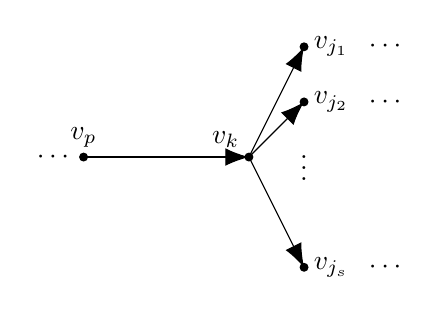
\begin{tikzpicture}[scale=0.7]
\coordinate (a) at (0,0);
\coordinate (b) at (3,0);
\coordinate (c) at (4,2);
\coordinate (d) at (4,1);
\coordinate (e) at (4,-2);
\coordinate (f) at (4,0.5);

\coordinate (g) at (5,2);
\coordinate (h) at (5,1);
\coordinate (i) at (5,-2);
\coordinate (j) at (0,0);


\draw (a) node[above]{$v_p$};
\draw (b) node[above left]{$v_k$};
\draw (c) node[right]{$v_{j_1}$};
\draw (d) node[right]{$v_{j_2}$};
\draw (f) node[below]{$\vdots$};
\draw (e)node[right]{$v_{j_s}$};

\draw (g)node[right]{$\cdots $};
\draw (h)node[right]{$\cdots $};
\draw (i)node[right]{$\cdots $};
\draw (j)node[left]{$\cdots $};

\draw [fill=black] (a) circle[radius=2pt];
\draw [fill=black] (b) circle[radius=2pt];
\draw [fill=black] (c) circle[radius=2pt];
\draw [fill=black] (d) circle[radius=2pt];
\draw [fill=black] (e) circle[radius=2pt];

\draw [-{Latex[length=3mm]}] (a)--(b) ;
\draw [-{Latex[length=3mm]}] (b)--(c) ;
\draw [-{Latex[length=3mm]}] (b)--(d) ;
\draw [-{Latex[length=3mm]}] (b)--(e) ;

\end{tikzpicture} 
\caption{Neighbors of vertex $v_k$.}
\label{fig:subgr}
\end{figure}


 \bigskip

 Proof of Observation: The equation in $\tilde{L}_Tx=e_k$ corresponding to vertex $v_k$  is 
 %
 \[
     (s+2)x_k-x_p-\sum_{r=1}^s x_{j_r}=0.
 \]
 %
  This gives 
  \[
  \begin{array}{rl} \vspace{0.2cm}
         x_p&=(s+2)x_k-\sum_{r=1}^s x_{j_r} \\ \vspace{0.2cm}
               &\ge (s+2)x_k-\sum_{r=1}^s (1/2)x_k \\ \vspace{0.2cm}
               &= (s/2+2)x_k  \\ \vspace{0.2cm}
               &\ge 2x_k
  \end{array}       
 \]
 %
 which proves the observation. 
 
 Consider now a directed edge $(v_p,v_k)$ in $T$.  We say that this edge is {\em good} if $x_p \ge 2 x_k$.
 
\smallskip
 {\em Claim: Every directed edge $(v_p,v_k)$ in $T$ is good.}
 
 \smallskip
 Proof of Claim: If $(v_p,v_k)$ is such that $v_k$ is a pendant vertex, then, by Lemma
 \ref{lem:pendant}, $x_p = 2 x_k$, so $(v_p,v_k)$ is good. Next, consider an edge $(v_{\ell},v_p)$, such every outgoing edge of $v_p$ is good. Then, by the Observation, $x_\ell \ge  2 x_p$, so also the edge $(v_{\ell},v_p)$ is good. We continue like this, and can thereby continue until all edges are covered, and they are all good, as desired. 
 
 Finally, the Claim directly gives the monotonicity property (\ref{eq:tree-d-mon}), which completes the proof.
 \end{proof}

From this theorem we conclude that the entries in each row $i$ of $B_T$ drop off exponentially fast as a function of the (combinatorial) distance from the vertex $v_i$.  
 In the case of a path, from the proof of the Observation in the above proof, we have $x_p \geq \frac{5}{2} x_k.$ This lower bound is tighter to $x_p$ than the one found in Theorem \ref{thm:B_monotone}.

With these results in hand, we now turn our attention to the main diagonal of doubly stochastic matrices.

Consider a tree $T$. Define $d(v_i,v_j)$ as the (combinatorial) {\em distance} between vertices $v_i$ and $v_j$, i.e., the number of edges in the unique $v_iv_j$-path in $T$.

The next result provides a lower bound on the diagonal entries of doubly stochastic matrices constructed from trees, as below.

\begin{corollary}
 \label{cor:tree_B_monotone}
  Let $T$ be a tree with $n$ vertices and let $B_T=[b_{ij}]=\tilde{L}_T^{-1}$.  Then 
  %
  \begin{equation}
   \label{eq:diag-L-ds}
     b_{ii} \ge \frac{1}{\sum_j 2^{-d(v_i,v_j)}}   \;\;\;\;(1\le i\le n). 
   \end{equation}
 % 
\end{corollary}
%
%\textcolor{red}{HERE}
\begin{proof}
 We fix vertex $v_i$ as stated above. Consider a vertex $v_j$ and the (unique) $v_iv_j$-path
 %
 \[
    v_{i_0}, v_{i_1}, v_{i_2}, \ldots, v_{i_k}
 \]
 %
 where $k=d(v_i,v_j)$, and $i_0=i$, $i_k=j$. 
 Theorem \ref{thm:tree_B_monotone} with repeated application of the inequality (\ref{eq:tree-d-mon}) gives
 \[
      b_{ii} \ge 2 \,b_{i,i_1} \ge 2^2 \,b_{i,i_2} \ge \cdots \ge 2^k \,b_{i,i_k} .
 \]     
 %
 Therefore 
 \[
    b_{ii} \ge 2^{d(v_i,v_j)} \,b_{ij} \;\;\;(1 \le j \le n).
 \]
 %
   
 Since $B$ is doubly stochastic its row sums are 1, so
 %
 \[
   1 = \sum_{j} b_{ij} \le \sum_j (2^{-d(v_i,v_j)}\, b_{ii})=b_{ii} \,\sum_j 2^{-d(v_i,v_j)}
 \]
 %
 which gives the desired inequality.
\end{proof}
\medskip

\begin{example}
{\rm 
Let $G=Br(k, \ell)$ be the so-called broom tree which is obtained from a path $P_k$ with $k$ vertices by adding $\ell$ vertices and attaching each of these to the same end vertex of the path.
We let the vertices of $P_k$ be labeled $1, 2, \ldots, k$ and the remaining vertices are labeled  by $k+1, k+2, \ldots, k+\ell$. In Fig.~\ref{fig_broom_tree_revision} the graph $Br(6, 5)$ is shown.
%
\begin{figure}[h]
\centering
\begin{minipage}{0.5\textwidth}
\centering

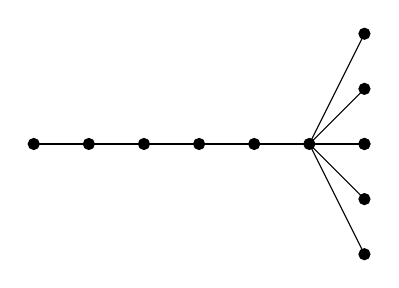
\begin{tikzpicture}[scale=0.7]
  \draw[fill] (0,0) circle(0.1cm);
  \draw[fill]  (1,0) circle (0.1cm);
  \draw[fill]  (2,0) circle (0.1cm);
  \draw[fill]  (3,0) circle (0.1cm);
  \draw[fill]  (4,0) circle (0.1cm);
   \draw[fill]  (5,0) circle (0.1cm);
 % \draw[fill]  (6,0) circle (0.2cm);
  \draw[fill]  (6,0) circle (0.1cm);     
  %
  \draw[fill]  (6,-1) circle (0.1cm);
  \draw[fill]  (6,0) circle (0.1cm);
 \draw[fill]  (6, 1) circle (0.1cm);
 \draw[fill]  (6, 2) circle (0.1cm);
 \draw[fill]  (6, -2) circle (0.1cm);
 % \draw (3,0.5) node{\tiny{$v_{ s}$}};
 % \draw (0,0.5) node{\footnotesize{$v_{1}$}};

%EDGES
\draw(0,0) --(1,0);
\draw(1,0) --(2,0);
\draw(2,0) --(3,0);
\draw(3,0) --(4,0);
\draw(4,0) --(5,0);
\draw(5,0) --(6,0);
\draw (5,0)--(6,-1);
\draw (5,0)--(6,1);
\draw (5,0)--(6,2);
\draw (5,0)--(6,-2);


 \end{tikzpicture}
\caption{Broom tree $Br(6, 5)$.}
\label{fig_broom_tree_revision}
\end{minipage}
\end{figure} 


The lower bound ($\ref{eq:diag-L-ds}$) in Corollary \ref{eq:diag-L-ds} for the diagonal entries of $B_G$ are 

\begin{eqnarray*}
%b_{11} &\geq & \frac{1}{ 2+(\ell-2) (\frac{1}{2} )^k}\\
b_{pp} & \geq & \frac{1}{3-(\frac{1}{2})^{p-1} +(\ell-2) (\frac{1}{2})^{k-p+1}
} \mbox{\, if \, \,} 1 \leq p\leq k,\\
%b_{kk} &\geq &\frac{1}{2- (\frac{1}{2})^{k-1} + \frac{\ell}{2}}\\
b_{k+q, k+q}& \geq &\frac{1}{
\frac{7}{4} + \frac{\ell}{4} -(\frac{1}{2})^{k}}, \mbox{\, if \, \,} 1\leq q\leq \ell.
\end{eqnarray*}

%The lower bound for $b_{11}$ comes from:
%$$\sum_j 2^{-d(v_1,v_j)}= 2^0+ 2^{-1}+ 2^{-2} + \ldots + 2^{-(k-1)} + \ell 2^{-k}= 2+ 
%(\ell-2) \left(\frac{1}{2}\right)^k.$$
Here the lower bound for $b_{pp}, 1\leq p\leq k$ comes from:
\begin{eqnarray*}    
\sum_j 2^{-d(v_p,v_j)}&= &
2^{-(p-1)}+ 2^{-(p-2)}+ \cdots+2^{-1}+2^0+ 2^{-1}+ 2^{-2}+ \cdots+ 2^{-(k-p)}+ \ell 2^{-(k-p+1)}\\
&=& 3-(\frac{1}{2})^{p-1}+ (\ell-2) \left(\frac{1}{2}\right)^{k-p+1}.\\
\end{eqnarray*}
%The lower bound for $b_{kk}$ comes from: 
%\begin{eqnarray*}    
%\sum_j 2^{-d(v_i,v_j)}&= &
%2^{-(k-1)}+ 2^{-(k-2)}+ \cdots+2^{-1}+2^0+ \ell 2^{-1}\\
%&=& 2- \left(\frac{1}{2}\right)^{k-1} + \frac{\ell}{2}.
%\end{eqnarray*}
Similarly, concerning the lower bound for $b_{k+q, k+q},$ with $1\leq q\leq \ell,$
we have 
\begin{eqnarray*}    
\sum_j 2^{-d(v_{p+q},v_j)}&= &
2^{-k}+ 2^{-(k-1)}+ \cdots+2^{-1}+2^0+ (\ell-1) 2^{-2}\\
&= & \frac{7}{4} -\left(\frac{1}{2}\right)^{k}+ \frac{\ell}{4}.
\end{eqnarray*}\hfill{$\diamond$}
}
    \end{example}


We now consider a general graph $G$. The goal is to establish a monotonicity property for the inverse matrix $B_G=\tilde{L}_G^{-1}$.  Let $d_j$ denote the degree of vertex $v_j$. 



\begin{theorem}
 \label{thm:G_B_monotone}
  Let $G$ be a connected graph and let $B_G=[b_{ij}]=\tilde{L}_G^{-1}$. Consider a vertex $v_i$ in $G$. Let $v_j$ be a vertex different from $v_i$. 
  
  Then there exists a $v_jv_i$-path $P=v_j, v_{j_1}, v_{j_2}, \ldots, v_{j_k}, v_i$ such that the entries in row $i$ of $B_G$ are monotone in the following sense 
  %
  \begin{equation}
    \label{eq:G-mon}
      b_{ij} < b_{i,j_1} < \cdots < b_{i,j_k} < b_{ii}. 
  \end{equation}

 In particular, $b_{ii}>b_{ij}$. So each diagonal element in $B_G$ is strictly largest in its row and column.
\end{theorem}
%
\begin{proof}
 Since $j \not = i$, the corresponding equation from $\tilde{L}_G x=e_i$ is 
 %
 \[
     x_j=\frac{1}{d_j+1}\sum_{k:\, v_k \sim v_j} x_k. 
 \]
  %
 Recall that  $v_k \sim v_j$ means that $v_k$ and $v_j$ are adjacent. Therefore  
 %
 \[
     x_j=\frac{1}{d_j+1}\sum_{k:\, v_k \sim v_j} x_k <\frac{1}{d_j}\sum_{k:\, v_k \sim v_j} x_k,
 \]
  %
  where the last expression is the average $x$-value among the neighbors of vertex $v_j$. (Note, concerning the inequality, we already know that every entry in the matrix $B$ is strictly positive.) Therefore there must be a  neighbor $v_{j_1}$ of $v_j$, i.e., $v_j \sim v_{j_1}$, with $x_j<x_{j_1}$.
 We repeat this calculation and argument with $j$ replaced by $j_1$. So there is a neighbor $v_{j_2}$ of $v_{j_1}$ such that $x_{j_1}<x_{j_2}$. Continuing like this we construct a path $P=v_j, v_{j_1}, v_{j_2}, \ldots, v_{j_k}, v_i$ with
  \[
   x_j<x_{j_1} < x_{j_2} < \cdots < x_{j_k}<x_i.
  \]
   %
   All the vertices in $P$ must be distinct as the $x$-value is strictly increased in each step. The process can only terminate in vertex $v_i$ because in any other vertex we can find a neighbor with higher $x$-value. This proves the theorem. 
\end{proof}

Concerning Theorem \ref{thm:G_B_monotone} the inequality $b_{ii}>b_{ij}$ was also shown in \cite[Theorem 2]{Merris_II}  with a different argument (and the equality case was discussed). The  ``path inequalities''  (\ref{eq:G-mon}) give a stronger result of a more global character. 


\section{Algorithm for trees and applications}
\label{sec:alg_tree}

The construction in the proofs of the previous subsection has a further potential which is to give a rather simple procedure for computing the inverse matrix $B_T=(\tilde{L}_T)^{-1}$ when $T$ is a tree. We discuss the details next. 

Let $T=(V,E)$ be a tree and label again its vertices by $v_1, v_2, \ldots, v_n$. Let $T^{(i)}$ be the directed tree obtained from $T$ by directing each edge away from the vertex $v_i$ ($i \le n$). We call $v_i$ the {\em root}  of $T^{(i)}$, and it is the unique vertex with no ingoing edge.
Let $\delta^+(v_k)$ denote the set of outgoing edges from vertex $v_k$, i.e., all tree edges of the form $(v_k,v_s)$ for some $s$. As usual $d_k$ is the degree of vertex $v_k$ in $T$.

Let $i \le n$ be fixed. The  following algorithm works on the tree $T^{(i)}$ with its root $v_i$. It computes edge labels, called {\em multipliers}, from the leaves towards the root $v_i$, and uses these multipliers to compute the $i$'th column $x$ in $B_T=(\tilde{L}_T)^{-1}$. 
For an edge $(v_p,v_k)$ the multiplier $m_{pk}$ will become 
 $m_{pk}=x_p/x_k$, so therefore  $x_p=m_{pk}x_k$.
The initial step is to consider the Laplacian equation for each pendent vertex, which relates the two values $x_p$ and $x_k$ where $v_k$ is the pendent vertex: $x_p=2x_k$. This gives the multiplier 2 for the edge $(v_p,v_k)$. 

Then, recursively,  we consider another edge $(v_p,v_k)$ where all multipliers have been determined for edges in $\delta^+(v_k)$, and consider the Laplacian equation for vertex $v_k$. This  gives a new multiplier for this edge $(v_p,v_k)$ which relates the values $x_p$ and $x_k$. Overall this gives a procedure where multipliers are computed from the leaves towards the root vertex $v_i$. Then the value $x_i$ may be determined (using that the row sum is 1), and, finally, all other values can be computed from the multipliers.  

\bigskip\bigskip\bigskip
{\small
\begin{tabbing}
{\bf Algor}\={\bf ithm $B_T$.} \\
Input: A tree $T$ and a vertex $v_i$ in $T$. 
\\
\\

 \>0. Construct the directed tree $T^{(i)}$.\\
 \>1. \=For each directed edge $(v_p,v_k)$ where $k\not =i$ and $v_k$ is a pendant vertex define the \\
   \>\>label $m_{pk}=2$. \\
 \>2. \>(a) Choose a directed edge $(v_p,v_k)$ where each edge in $\delta^+(v_k)$ has been \\
 \>\>labeled. Then give \=the edge $(v_p,v_k)$ the label \\
 \>\> \>         $m_{pk}=d_k+1-\sum_{j:(v_k,v_j)\in \delta^+(v_k)} 1/m_{kj}$. \\
 \>\>(b) Repeat step (a) until all edges have been labeled.  \\ 
\>3. (a) Let \\
\>\>\> $x_i=(d_i+1-\sum_{j:(v_i,v_j)\in \delta^+(v_i)} 1/m_{ij})^{-1}$. \\
\>\>(b) For  each directed edge $(v_p,v_k)$ where $x_p$ has been computed, let \\
\>\>\> $x_k=x_p/m_{pk}$.   \\

\\
Output: $x$, which is the $i$'th column  in $B_T=(\tilde{L}_T)^{-1}$. 
\end{tabbing}
}

\medskip
\begin{theorem}
 \label{thm:tree_alg_BT}
  Let $T$ be a tree with $n$ vertices. Algorithm $B_T$ correctly computes the $i$'th column $x$ in $B=(\tilde{L}_T)^{-1}$.  The number of steps is $O(n)$. This gives an $O(n^2)$ algorithm to compute $B_T$.
  
\end{theorem}
%
\begin{proof}
Let $x$ denote the $i$'th column of $B_T=(\tilde{L}_T)^{-1}$. Consider the directed tree $T^{(i)}$ and for each directed edge $(v_p,v_k)$ define 
 %
 \[
    m^*_{pk}=x_p/x_k.
 \]
 
 We claim that $m_{pk}=m^*_{pk}$ for each $(v_p,v_k)$, where $m_{pk}$ is determined by Algorithm $B_T$. First, consider the case when $(v_p,v_k)$ is such that $v_k$ is a pendant vertex and $p\not =i$. Then, the Laplace equation associated with vertex $v_k$ is 
 $2x_k=x_p$, so 
 %
 \[
    m^*_{pk}=x_p/x_k=2=m_{pk},
 \]
 %
 as desired. Next, consider $(v_p,v_k)$ where $v_k$ is not a pendant vertex and $p \not =i$. Assume that $m^*_{kj}=m_{kj}$ for each $(v_k,v_j) \in \delta^+(v_k)$. Then the Laplace equation for vertex $v_k$ is 
 %
 \[
 \begin{array}{ll}\vspace{0.2cm}
    (d_k+1)x_k&=x_p+\sum_{(v_k,v_j) \in \delta^+(v_k)} x_j\\ \vspace{0.2cm}
     &=x_p+\sum_{(v_k,v_j) \in \delta^+(v_k)} x_k/m^*_{kj} \\ \vspace{0.2cm}
     &=x_p+\sum_{(v_k,v_j) \in \delta^+(v_k)} x_k/m_{kj}.
 \end{array}
 \]
 %
 Therefore
 \[
  \big(d_k+1-\sum_{(v_k,v_j) \in \delta^+(v_k)} 1/m_{kj}\big)x_k=x_p 
 \]
 which means, by Step 3(a) in Algorithm $B_T$ that
 $m_{pk}x_k=x_p$. So 
 %
 \[
    m^*_{pk}=x_p/x_k=m_{pk}.
 \]
 %
 Finally, consider vertex $v_i$. The corresponding Laplace equation gives the expression for $x_i$ in Step 3(a). Then, the remaining values $x_k$ ($k \not = i)$ are computed as in Step 3(b), as $m^*_{pk}=x_p/x_k=m_{pk}$. 

 

\end{proof}
 
Thus Algorithm $B_T$ traverses the edge set of $T$ twice. The first time from leaves towards the root, in order to compute the multipliers $m_{kp}$. The second time one traverses from the root in, e.g.,  a breadth-first-search way and compute the desired vector $x$.

For small, or some simple classes of trees, Algorithm $B_T$ may be preformed analytically and provide an explicit expression for the inverse matrix $B_T$.
We give some such examples next.

\begin{example} 
{\rm 
We will apply Algorithm $B_T$ to the tree $T$ depicted in Figure \ref{tree} computing its $6$'th column. So, let $i=6$.
Step 2 gives $m_{52}=m_{53}=m_{41}=2$ and then $m_{65}=3$, $m_{64}=5/2$. In Step 3 we first compute $x_6=(3-(1/3+2/5))^{-1}=15/34$, and using the multipliers we find $x_{5}= 5/34$, $x_{4} =3/17$, $x_{2}= x_{3}=5/68$ and $x_{1} =3/34$. Thus the $6$'th column, and row,  of the matrix $B_{T}$ is $x=(3/34, 5/68, 5/68, 3/17, 5/34, 15/34)=\frac{1}{68}(6,5,5,12,10,30)$.
}\hfill{$\diamond$}
\end{example} 

\begin{figure}
%\begin{minipage}[b]{.45\textwidth}
\centering
 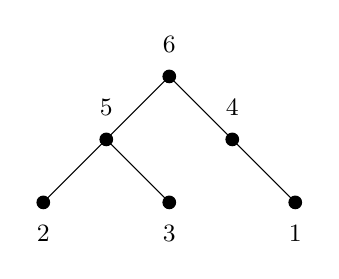
\begin{tikzpicture}[scale=0.4]
  \draw[fill]  (4,0) circle (0.2cm);
  \draw[fill]  (2,-2) circle (0.2cm);
 \draw[fill]  (6,-2) circle (0.2cm);
 \draw[fill]  (0,-4) circle (0.2cm);
 \draw[fill]  (4,-4) circle (0.2cm);
 \draw[fill]  (8,-4) circle (0.2cm);
 %NODES
 \draw  (4,1) node{\small{$6$}};
  \draw  (2,-1) node{\small{$5$}};
  \draw (6,-1) node{\small{$4$}};
   \draw (0,-5) node{\small{$2$}};
   \draw (4,-5) node{\small{$3$}};
   \draw[fill] (8,-5) node{\small{$1$}};
%EDGES
 \draw (4,0) --(2,-2);
 \draw (4,0) --(6,-2);
 \draw (2,-2) --(0,-4);
 \draw (2,-2) --(4,-4);
 \draw (6,-2) --(8,-4);
 \end{tikzpicture}
\caption{A tree $T$ with $6$ vertices}
\label{tree}
%\end{minipage}
\end{figure}


\begin{example}
{\rm    Let $S_n$ be the star with $n\geq 2$ vertices where the central vertex is labelled as $v_n$. Then  
    \begin{equation}\label{starinverse}
  B_{S_n}= \frac{1}{2n+2}\left[
  \begin{array}{ccccc}
    n+2& 1&\cdots& 1& 2 \\
   1& n+2&\cdots& 1& 2 \\
    && \ddots \\
    1& 1 &\cdots& n+2& 2 \\
   2& 2&\cdots& 2& 4 \\
  \end{array}
  \right].
  \end{equation}

To verify this we use Algorithm $B_T$ to compute the $i$'th column of $B_{S_n}$. 

First compute the last column of $B_{S_n}$. Step 1 gives $m_{nj}=2$ for $j\le n-1$, so Step 2 is not needed. Then Step 3 (a) gives  $x_n= (n-(n-1)(1/2))^{-1}= 2/ (n+1)$. Step 3 (b) gives $x_j=2/(2n+2)$ for $j<n$. 

Next,  compute the first column of $B_{S_n}$. Step 1 gives $m_{nj}=2$ for $2\le j \le n-1$, and Step 2 gives $m_{1n}=(n+2)/2$. Then Step 3 gives $x_1=(n+2)/(2n+2)$,  $x_n=2/(2n+2)$, and $x_j=1/(2n+2)$ for $2 \le j \le n-1$.
The other columns follow from column $1$, by symmetry.
}\hfill{$\diamond$}
\end{example}

Next, we consider paths. In the next example we will see that the entries of $B_{P_n}$ (in this case just for the last column) can be written as function of quotients of Fibonacci numbers.
%We refer that the smallest entry of $B_{P_n}$, $\omega(P_n)$, is stated in \cite[Theorem 2.1]{Zhang}. 


\begin{example}
{\rm 
 Consider the path $P_n=v_1, v_2, \ldots, v_n$. We compute the $n$'th column of the matrix $B_{P_n}.$  
Step 1 gives $m_{21}= 2=\frac{f_3}{f_1}.$
From Step 2, and 
%for each \textcolor{red}{$1 \leq \ell \leq n-2$, we have 
%$$m_{\ell+2, \ell+1} = 3- \frac{f_{2\ell-1}}{f_{2\ell +1}}= \frac{3f_{2\ell +1}- %f_{2\ell-1}}{f_{2\ell +1}} = \frac{f_{2\ell+3}}{f_{2\ell +1}}.$$}
for each $2\leq j\leq n-1$, we have 
$$m_{j+1, j} = 3- \frac{f_{2j-3}}{f_{2j -1}}= \frac{3f_{2j-1}- f_{2j-3}}{f_{2j-1}} = \frac{f_{2j+1}}{f_{2j-1}}.$$

From Step 3 (a) we have 
$x_n = ( 2 - \frac{f_{2n-3}}{f_{2n-1}})^{-1}=( \frac{2 f_{2n-1} -f_{2n-3}}{f_{2n-1}})^{-1} =\frac{f_{2n-1}}{f_{2n}}.$
From Step 3 (b), using the multipliers, we obtain $$x_{n-1}=(m_{n,n-1})^{-1} x_n =\frac{f_{2n-3}}{f_{2n-1}}x_{n}=\frac{f_{2n-3}}{f_{2n}},$$ and so on. The procedure is repeated until $x_1$ is obtained. 
Then, the $n$'th column of $B_{P_n}$ is 
\[
x= (1/f_{2n}) \cdot   (f_1, f_3,\ldots , f_{2n-3}, f_{2n-1})    
\] 
as confirmed in Section 3.
}\hfill{$\diamond$}
\end{example}

\begin{example}
{\rm
Let $n_1, n_2,  \ldots, n_{k-1}$ be positive integers. We compute the first column of $B_{S},$ where $S=S(n_1,n_2, \ldots, n_{k-1})$ is a starlike tree.  The starlike tree $S=S(n_1,n_2, \ldots, n_{k-1})$ is a tree that results from the stars $S_{n_{1}+1}$, \ldots, $S_{n_{k-1}+1}$ by connecting their centers to an extra vertex with label $1$. The neighbours of $1$ are labelled as $2,3, \ldots , k$. %\textcolor{red}{The neighbours of $2$ are $1$ and the pendant vertices labelled as $k+1, \ldots, k+ %n_1$, the neighbours of $3$ are $1$ and the vertices labelled as $k+n_{1} +1, \ldots, k+ n_{1} + %n_2$, and so on, so the neighbours of $k$ are $1$ and the vertices labelled as
%$ k+n_{1}+\cdots+ n_{k-2} +1, \ldots,k+ n_{1}+n_{2} + \cdots +n_{k-1}.$}
For $j= 2, \ldots, k$ the neighbours of $j$ are the vertex $1$ and the pendant vertices labelled as $ k+n_{1}+\cdots+ n_{j-2} +1, \ldots,k+ n_{1}+n_{2} + \cdots +n_{j-1},$ where the sum $n_{1}+\cdots+ n_{j-2}$ is void for $j=2.$
See Fig.~\ref{fig:starlike} for $S(n_1, n_2, n_3)=S(3,3,4).$\\
Using Algorithm $B_T$ we will now compute the first column of $B_S$.
%\textcolor{red}{Thus, Step 1 gives:
%$$m_{2, k+\ell_1}=2, 1\leq \ell_1 \leq n_{1},$$
%$$m_{3, k+n_{1}+\ell_{2}}=2, 1\leq \ell_{2} \leq n_{2},$$
%$$\vdots,$$
%$$m_{k, k+n_{1}+\cdots+ n_{k-2}+\ell_{k-1}}=2, 1\leq \ell_{k-1} \leq n_{k-1}. $$
%}
Thus for $j=2, \ldots, k$, Step 1 gives
$$m_{j, k+n_{1}+\cdots+ n_{j-2}+\ell_{j-1}}=2, \;\;(1\leq \ell_{j-1} \leq n_{j-1}), $$ where  $n_{1}+\cdots+ n_{j-2}$ is void for $j=2.$
%
\\
%\begin{tabular}{r|r|r|r}
%$\begin{array}{ccc}
%    m_{2,k+1}&=& 2 \\
%    m_{2, k+2} &=& 2\\
%    &\vdots&\\
 %   m_{2,k+n_1}&=& 2 
%    \end{array}$
%& 
%$
%\begin{array}{ccc}
%   m_{3, k+n_{1}+1}&=&2  \\
%    x_{3,k+n_{1}+ 2} &=&2\\
%    &\vdots&\\
%    x_{3, k+n_{1} +n_{2}} &= &2 
%    \end{array}
%    $
%    & 
%   $ \cdots $ 
%    &
%    $
%    \begin{array}{ccc}
%    m_{k,k+n_{1}+\cdots+n_{k-2} +1} &= & 2  \\
%    m_{k,k+n_{1}+\cdots+n_{k-2}+ 2} &= & 2 \\
%    &\vdots&\\
%    m_{k, k+n_{1}+\cdots+n_{k-2}+ n_{k-1}}&=& 2 
%    \end{array}
%    $
%\end{tabular}
%\bigskip\\

Step 2 gives: $ m_{1, \ell},$ with $2 \leq \ell \leq k$, 
$m_{1, \ell} = n_{\ell-1} +2 - (n_{\ell-1}) \frac{1}{2}= \frac{n_{\ell-1} +4}{2}.\bigskip$

From Step 3 (a) we have: 
$x_1 = (k- (\frac{2}{n_{1}+4} + \frac{2}{n_{2}+4}+\cdots+ \frac{2}{n_{k-1}+4}))^{-1}= \gamma.$
Then, from (b) we have $x_j =\frac{2}{n_{j-1}+4} x_{1}= \frac{2}{n_{j-1}+4} \gamma,$ with $2 \leq j\leq k,$
%\begin{eqnarray*}
%x_2 =\frac{2}{n_{2}+4} x_{1}, x_3  = \frac{2}%{n_{3}+4} x_{1}, \ldots, x_k =\frac{2}{n_{k}+4} x_{1};
%\end{eqnarray*}
and
$$
\begin{array}{lllllllll}
x_{k+1}&= &x_{k+2}&= & \ldots&= &x_{k+n_1}&=& \frac{1}{n_1+4} \gamma;\\
x_{k+n_1 +1}& = &x_{k+n_1 +2}& =& \ldots &=& x_{k+n_1 +n_2}& = &\frac{1}{n_2+4} \gamma; \\
&\vdots& & & & & & &\\
x_{k+n_1 +\cdots+ n_{k-2}+1} &= &
x_{k+n_1 +\cdots+ n_{k-2}+2}& =& \ldots &=& x_{k+n_1 +\cdots+n_{k-2}+ n_{k-1}} &=& \frac{1}{n_{k-1}+4} \gamma.
\end{array}
$$
Thus, the 1st column of $B_{S}$ is:
$$
(\gamma, \frac{2}{n_1 +4}\gamma, \ldots, \frac{2}{n_{k-1} +4}\gamma,\underbrace{\frac{1}{n_1+4}\gamma, \ldots, \frac{1}{n_1+4} \gamma}_{n_1}, \ldots, \underbrace{\frac{1}{n_{k-1}+4} \gamma, \ldots, \frac{1}{n_{k-1}+4} \gamma}_{n_{k-1}} ).
$$
}
\end{example} \hfill{$\diamond$}

\begin{figure}
\centering
 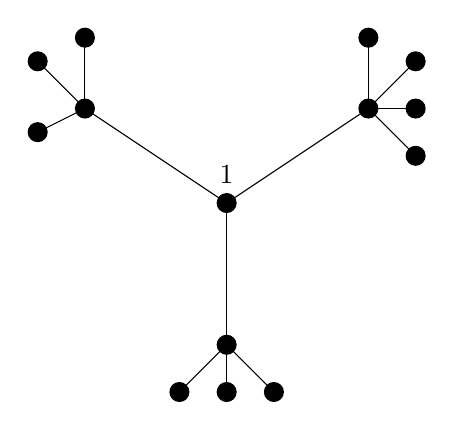
\begin{tikzpicture}[scale=0.6]
  \draw[fill]  (0,0) circle (0.2cm);
  \draw[fill]  (-3,2) circle (0.2cm);
 \draw[fill]  (3,2) circle (0.2cm);
\draw[fill]  (0,-3) circle (0.2cm);
\draw[fill]  (0,-4) circle (0.2cm);
\draw[fill]  (1,-4) circle (0.2cm);
\draw[fill]  (-1,-4) circle (0.2cm);  
\draw[fill]  (4,3) circle (0.2cm);
\draw[fill]  (4,1) circle (0.2cm);
\draw[fill]  (4,2) circle (0.2cm);
\draw[fill] (3,3.5) circle (0.2cm);
    
  
\draw[fill]  (-4,3) circle (0.2cm);
\draw[fill]  (-3,3.5) circle (0.2cm);
\draw[fill]  (-4,1.5) circle (0.2cm);
 
%NODES
 \draw  (0,0.6) node{$1$};
%EDGES
% \draw (0,0) --(-3,-2);
  \draw (0,0) --(-3,2);
  \draw (0,0) --(3,2);
  \draw (0,0) --(0,-3);
  
  \draw (0,-3) --(0,-4);
  \draw (0,-3) --(1,-4);
  \draw (0,-3) --(-1,-4);
    
  \draw (3,2) --(4,3);
  \draw(-3,2)--(-4,3);
  \draw(-3,2)--(-3,3.5);
  \draw(-3,2)--(-4,1.5);       
  \draw(3,2)--(4,1);
  \draw(3,2)--(3,3.5);  
    \draw(3,2)--(4,2); 
\end{tikzpicture} 
\caption{S(3,3,4)}
\label{fig:starlike}
\end{figure}

\medskip
We return to general trees and we will now give a rough estimate of the multipliers in Algorithm $B_T$. If $v_k$ is a pendent vertex, then its incident edge $(v_p,v_k)$ is called a {\em pendent edge}.  

\begin{theorem}
  \label{thm:mult-prop}
  Consider a tree $T$. Let $i \le n$ and consider the multipliers $m_{pk}$ in Algorithm $B_T$. For each edge $(v_p,v_k)$ the following inequalities hold 
  %
  \begin{equation}
    \label{eq:B-ineq}
     2 \le (1/2)d_k+3/2 \le m_{pk} \le d_k+1.
  \end{equation}
  %
  If $(v_p,v_k)$ is a pendent edge, equality holds throughout, so $m_{pk}=2$.
\end{theorem}
%
\begin{proof}
 If $(v_p,v_k)$ is a pendent edge, then $m_{pk}=2$ by Lemma \ref{lem:pendant}.  Next, consider an edge $(v_p,v_k)$ where $v_k$ is non-pendent, so $d_k\ge 2$.  
 Assume that 
 %
 \[
     2 \le  m_{kj} \le d_j+1 \;\;\; \mbox{\rm for all $j$ with $(v_k,v_j) \in \delta^+(v_k)$.}
 \]
 Then, from Algorithm $B_T$, we have 
 %
 \[
 \begin{array}{ll} \vspace{0.2cm}
    d_k+1\ge m_{pk}&=d_k+1-\sum_{j:(v_k,v_j)\in \delta^+(v_k)} 1/m_{kj} \\ \vspace{0.2cm}
       &\ge d_k+1-\sum_{j:(v_k,v_j)\in \delta^+(v_k)} 1/2 \\ \vspace{0.2cm}
       &= d_k+1-(1/2)(d_k-1) \\ \vspace{0.2cm}
       &=(1/2)d_k+3/2 \\ \vspace{0.2cm}
       &\ge 2.
 \end{array}   
 \]
 %
 So, the result now follows by induction by considering edges in a sequence from pendent vertices up to the edge $(v_p,v_k)$.
\end{proof}

The previous theorem gives bounds on the change among the entries in $B=[b_{ij}]$ when one moves from a pendent vertex towards vertex $i$ (which gives number of row/column $i$ in $B$). We see from the proof that the lower bound on $m_{pk}$ is tight if and only if $v_j$ is a pendant vertex for each $(v_k,v_j) \in \delta^+(v_k)$.

\begin{corollary}
  \label{cor:mult-prop3}
  Let $T$ be a tree and let $i \le n$. Consider an edge $(v_p,v_k)$ in $T^{(i)}$ and define 
  \[
     m^*=\min\{m_{kj}: (v_k,v_j) \in \delta^+(v_k)\}.
  \]
  Then 
  %
  \begin{equation}
  \label{eq:B-ineq2}
      m_{pk} \ge (1-1/m^*)d_k+1+1/m^*.
  \end{equation}
  %
 
\end{corollary}

\begin{proof}
 As in the previous proof, from Algorithm $B_T$, we get 
 %
 \[
 \begin{array}{ll} \vspace{0.2cm}
    m_{pk}&=d_k+1-\sum_{j:(v_k,v_j)\in \delta^+(v_k)} 1/m_{kj} \\ \vspace{0.2cm}
       &\ge d_k+1-\sum_{j:(v_k,v_j)\in \delta^+(v_k)} 1/m^* \\ \vspace{0.2cm}
       &= d_k+1-(1/m^*)(d_k-1) \\ \vspace{0.2cm}
       &=(1-1/m^*)d_k+1+1/m^*.
 \end{array}   
 \]
 %
 \end{proof}


From Theorem \ref{thm:mult-prop} and Corollary \ref{cor:mult-prop3} we see that if the multipliers are ``large'' for all multipliers of outgoing edges of a vertex $v_k$, then the next multiplier $m_{pk}$ will be close to the degree $d_k$. 


\medskip
As an application of the results above, we consider a special class of trees. Let $\mc{T}^{(3)}_n$ be the class of trees where each non-pendent vertex has degree $3$ (also called regular tree of degree $3$). These are a special case of {\em chemical trees}, i.e., trees that have no vertex with degree greater than $4$. Chemical trees are used to represent chemical structures and they offer a powerful way to understand and analyze chemical compounds.
Let $T \in\mc{T}^{(3)}_n$ and consider its vertices $v_1, v_2, \ldots, v_n$. Let $i,j \le n$ with $i \not = j$. We let $d(i,j)$ denote the distance between $v_i$ and $v_j$, defined as the number of edges in the (unique) $v_iv_j$-path. Also, let $V_p$ denote the set of pendent vertices in $T$. Define for $i \not = j$ 
%
\begin{equation}
 \label{eq:deg3-bd}  
\begin{array}{l}\vspace{0.4cm}
\tilde{\eta}(i,j)=
\left\{
\begin{array}{cr}
   (1/4)^{d(i,j)} &\mbox{if $v_j \not \in V_p$,} \\ 
   (1/2)\cdot (1/4)^{d(i,j)-1} &\mbox{if $v_j  \in V_p$;}
\end{array}
\right.
\\
\hat{\eta}(i,j)=
\left\{
\begin{array}{cr}
   (1/3)^{d(i,j)} &\mbox{if $v_j \not \in V_p$,} \\ 
   (1/2)\cdot (1/3)^{d(i,j)-1} &\mbox{if $v_j  \in V_p$.}
\end{array}
\right.
\end{array}
\end{equation}

\begin{corollary}
  \label{cor:3-trees}
  Let $T \in\mc{T}^{(3)}_n$ and consider $B_T=[b_{ij}]$. Let $i \le n$. Then 
  %
  \begin{equation}
    \label{eq:T3-bounds} 
    \big(1+\sum_{j\not = i} \hat{\eta}(i,j) \big)^{-1} \le 
    b_{ii} \le \big(1+\sum_{j\not = i} \tilde{\eta}(i,j) \big)^{-1},
  \end{equation}
  and for $j \not = i$
    \begin{equation}
    \label{eq:T3-bounds2} 
    \tilde{\eta}(i,j)\big(1+\sum_{k\not = i} \bar{\eta}(i,k) \big)^{-1} 
    \le 
    b_{ij} \le \hat{\eta}(i,j)\big(1+\sum_{k\not = i} \tilde{\eta}(i,k) \big)^{-1}.
  \end{equation}
 %
\end{corollary}

%
\begin{proof}
  Let $j \not = i$. Let the unique $v_iv_j$-path be 
  \[
    v_i, v_{i_1}, v_{i_2}, \ldots, v_{i_{t-1}}, v_j  
  \]
%
where $d(i,j)=t$. By the definition of multipliers $m_{pk}$ we obtain 
  \[
    b_{ij}=b_{ii} \cdot m_{ii_1}^{-1}m_{i_1i_2}^{-1} \cdots m_{i_{t-1}j}^{-1}  
  \]
%
 where we suppress the dependence of $j$ in the intermediate vertices.  Now, for an edge incident to a pendent edge, the multiplier is 2. Otherwise, as degrees for non-pendent vertices are $3$, it follows from Theorem \ref{thm:mult-prop} that
 %
 \[
     3 \le m_{pk} \le 4.
 \]
 %
 This gives
 \begin{equation}
  \label{eq:bii_rel}   
   1=\sum_j b_{ij}=b_{ii}+b_{ii}\sum_{j \not = i} m_{ii_1}^{-1}m_{i_1i_2}^{-1} \cdots m_{i_{t-1}j}^{-1}
 \end{equation}
 %
 and by using the lower and upper bounds for the multipliers, one obtains (\ref{eq:T3-bounds}). Then  (\ref{eq:T3-bounds2}) also follows. 
\end{proof}


To close this section, we briefly discuss a centrality concept in graphs. 
As presented in \cite{Merris_II}, and proved in \cite{Chebotarev}, for a graph $G$ and the matrix $B_G=(\tilde{L}_G)^{-1}=[b_{ij}]$, the function 
\[
  \rho(v_i,v_j)=b_{ii}+b_{jj}-2b_{ij}
\]
%
gives a metric on $V$. Moreover (see \cite{Merris_II}),   
$r(i):=\sum_{j=1}^n \rho(v_i,v_j)$ ($i \le n$)
is minimized if and only if $b_{ii}$ is a minimum. Such a minimizing vertex  $v_i$  was called a {\em least remote vertex}. This suggests that diagonal entries that are small correspond to ``central'' vertices in the graph. 

For a tree $T$, this observation can also be seen heuristically from (\ref{eq:bii_rel}). In fact, small value of $b_{ii}$ corresponds to a large value of the last sum in (\ref{eq:bii_rel}) which (as $m_{pk}\ge 2$) typically happens for a vertex $v_i$ with ``many vertices close'' (close in terms of combinatorial distance in $T$). This is a property of central vertices in a tree. We leave it for further work to study these questions, and, hopefully, to prove interesting results relating $b_{ii}$ to combinatorial center concepts. 




   \begin{figure}[ht]
    \begin{center}
    \vspace{-3.5cm}
	\includegraphics[width=10cm]{tree1.pdf}
    \vspace{-4.5cm}
    \end{center}
    \caption{A tree $T$.}
    \label{fig:tree1}
    \end{figure}
  
   \begin{example}
 \label{ex:tree_dist_bii}
    {\rm 
    Let $n=10$ and consider the tree $T$ in Fig.~\ref{fig:tree1}. Vertex $v_i$ is indicated by the label $i$. The matrix $B_T$ is shown below where the diagonal is indicated in boldface.
   
{\scriptsize 
\[
B_T =
\left[
\begin{array}{rrrrrrrrrr}
    {\bf 0.3723} & 0.1861 & 0.1168 & 0.0365 & 0.0146 &   0.0584 &   0.0073  &  0.1861&    0.0146&    0.0073\\
    0.1861 & {\bf 0.5931} & 0.0584 & 0.0182 & 0.0073 &   0.0292 &   0.0036  &  0.0931&    0.0073&    0.0036\\
    0.1168 & 0.0584 & {\bf 0.3504} & 0.1095 & 0.0438 &   0.1752 &   0.0219  &  0.0584&    0.0438&    0.0219\\
    0.0365 & 0.0182 & 0.1095 & {\bf 0.3467} & 0.1387 &   0.0547 &   0.0693  &  0.0182&    0.1387&    0.0693\\
    0.0146 & 0.0073 & 0.0438 & 0.1387 & {\bf 0.4555} &   0.0219 &   0.2277  &  0.0073&    0.0555&    0.0277\\
    0.0584 & 0.0292 & 0.1752 & 0.0547 & 0.0219 &  {\bf  0.5876} &   0.0109  &  0.0292&    0.0219&    0.0109\\
    0.0073 & 0.0036 & 0.0219 & 0.0693 & 0.2277 &   0.0109 &  {\bf  0.6139}  &  0.0036&    0.0277&    0.0139\\
    0.1861 & 0.0931 & 0.0584 & 0.0182 & 0.0073 &   0.0292 &   0.0036  & {\bf  0.5931}&    0.0073&    0.0036\\
    0.0146 & 0.0073 & 0.0438 & 0.1387 & 0.0555 &   0.0219 &   0.0277  &  0.0073&   {\bf  0.4555}&    0.2277\\
    0.0073 & 0.0036 & 0.0219 & 0.0693 & 0.0277 &   0.0109 &   0.0139  &  0.0036&    0.2277&  {\bf 0.6139}
\end{array}
\right].
\]
}
The smallest entries are $b_{44}$ followed by $b_{33}$. 
This suggests that these vertices play a role as ``central" vertices in the graph. 
 

    }\hfill{$\diamond$}
\end{example}

\medskip
We remark that in \cite{GD07} distance vectors of  vertices in trees (vectors which contain the combinatorial distances of a vertex to all vertices in the tree) were used to define a partial order of vertices based on weak majorization of distance vectors. This was used to define a center concept, the majorization center, consisting of the ``smallest vectors'' in this majorization order. 
 In Example \ref{ex:tree_dist_bii} the majorization center consists of the vertices $v_3$ and $v_4$. 




\section{Heat equation, extensions and concluding remarks}

We now briefly discuss a connection to partial differential equations (PDE) and the relevance of our results above for this. The {\em heat equation} \cite{Ragnar2005} is a PDE with applications in heat diffusion and particle diffusion, and it also plays a role in mathematical finance. The discrete heat equation has the form 
\[
\frac{du}{dt}=L_G u, \;\; u(0)=u_0,
\]
where $L_G$ is the Laplacian matrix of a graph $G$ obtained by discretizing the domain. Here  $u(x,t)$ indicates the temperature in position $x$ (in some space) at time $t$, and $u_0$ is the initial condition (a function of $x$ at time zero). For more on the heat equation and the computational approach to PDEs, see \cite{Ragnar2005}. 

The formal solution of the heat equation is 
$u(t)=P(t)u_0$ where $P(t)$ is the matrix exponential $P(t)=e^{tL_G}$. This  leads to different computational methods for solving the heat equation (e.g., Taylor expansion or eigenvector methods). Observe that 
\[
   P(t)=e^{tL_G}=e^{-tI}e^{t\tilde{L}_G}
\]
which means that the matrix exponential of the modified Laplacian matrix of $G$ may be used computationally as a heat solver, followed by a simple diagonal matrix scaling. Moreover, an extension of $\tilde{L}_G$  is of interest in connection with an implicit Euler method for solving the discrete heat equation, as we now briefly describe. Consider a step $h>0$ and consider the linear equation 
%
\begin{equation}
\label{eq:heat_eq_k}
    (I+hL_G)u^{k+1}=u^k   
\end{equation}
%
for finding a new iterate $u^{k+1}$ based on the previous iterate $u^k$. Here the coefficient matrix is 
\[
    \tilde{L}_G^{h}:=I+hL_G
\]
which is positive definite, and therefore invertible. So the solution of (\ref{eq:heat_eq_k}) is $u^{k+1}=(\tilde{L}_G^{h})^{-1}u^k$. Note that for $h=1$, we have $\tilde{L}_G^{1}=\tilde{L}_G$ and $(\tilde{L}_G^{1})^{-1}=B_G$. 

Thus, the new matrix $\tilde{L}_G^{h}$ generalizes the modified Laplacian matrix $\tilde{L}_G$, and it arises in a natural way from the heat equation.

 $\tilde{L}^{h}_G$ is an M-matrix, and has a nonnegative inverse. The inverse is positive if $G$ is connected.  Moreover, $\tilde{L}^{h}_G$ has constant row and column sums, equal to $1$, so (when $e$ is the all ones vector)  
\[
  \tilde{L}^{h}_G e=e, \;\;\mbox{\rm and}\;\; 
  e^t \tilde{L}^{h}_G=e^t.
\]
 If we multiply by $(\tilde{L}^{h}_G)^{-1}$ in the previous equations, we obtain 
\[
    (\tilde{L}^{h}_G)^{-1} e=e \;\;\mbox{\rm and}\;\; 
    e^t(\tilde{L}^{h}_G)^{-1}=e^t.
\]

This shows that $(\tilde{L}^{h}_G)^{-1}$ is a doubly stochastic matrix.

Next, we comment on how our previous results may be extended to $(\tilde{L}^{h}_G)^{-1}$ where the proofs are very similar:

\begin{itemize}
 \item Lemma \ref{lem:pendant}: replace the factor 2 in (\ref{eq:B_pendant}) by $\frac{1+h}{h}$.
 \item Theorem \ref{thm:tree_B_monotone}: replace the factor 2 in (\ref{eq:tree-d-mon}) by $\frac{1+h}{h}$.  
 \item Corollary \ref{cor:tree_B_monotone}: replace the factor 2  in (\ref{eq:diag-L-ds}) by $\frac{1+h}{h}$.
 \item Theorem \ref{thm:G_B_monotone}: the statement of the theorem is the same. For $h$ small this means that the values in the off-diagonal entries drop very fast as a function of the distance to $v_i$ (diagonal vertex).
 \item Theorem \ref{thm:tree_alg_BT}: as before. Algorithm $B_T$ is modified as follows: 
 in Step 1, $m_{pk} = (1+h)/h$; 
 in Step 2(a) the modified multiplier is 
 \[
    m_{pk}=1/h+d_k-\sum_{j:(v_k,v_j)\in \delta^+(v_k)} 1/m_{kj},
 \]
 and in 3(a) the modified expression for $x_i$ is 
 \[
    x_i=(1/h+d_i-\sum_{j:(v_i,v_j)\in \delta^+(v_i)} 1/m_{ij})^{-1}.
 \]
 %
 \item Theorem \ref{thm:mult-prop}: replace (\ref{eq:B-ineq}) by 
 \[
      1+\frac{1}{h} \le (1-\frac{h}{h+1})d_k +\frac{h}{h+1} +\frac{1}{h}
      \le m_{pk} \le d_k+\frac{1}{h}. 
 \]
 %
 \end{itemize}

\bigskip\bigskip
Finally, as possible future work, we believe that it is interesting to further explore the connection and usefulness of these modified Laplacians for PDEs. 
Another interesting topic is to study combinatorial and geometric properties of the set of doubly stochastic matrices obtained as inverses of modified Laplacian matrices, as a subset of $\Omega_n$.


\bigskip\bigskip
{\bf Acknowledgments.} We thank Kenneth H. Karlsen for pointing out the connections to the heat equation and, more generally, the role of the discrete Laplacian in PDEs.  
Enide Andrade is supported by CIDMA under the
Portuguese Foundation for Science and Technology 
(FCT, https://ror.org/00snfqn58)  
Multi-Annual Financing Program for R\&D Units with project UID/PRR/4106/2025.


\begin{thebibliography}{99}

%\bibitem{EALCGD22}  E.~Andrade, L.~Ciardo,  G.~Dahl, %Perron Values and classes of  trees, \textit{Linear %Algebra Appl.}, 639 (2022), 135--158.
%\bibitem{EALCGD19}  E.~Andrade, L.~Ciardo,  G.~Dahl, % Combinatorial Perron parameters for trees, %\textit{Linear Algebra Appl.}, 566 (2019), 138--166.

%\bibitem{EAGD17} E.~Andrade,  G.~Dahl,  %Combinatorial Perron values of trees and bottleneck %matrices, \textit{Linear Multilinear Algebra} 65(12) %(2017), 2387--2405.

\bibitem{Berman} A. Berman, X.D. Zhang, A note on the degree antiregular graphs, {\em Linear Multilinear Algebra}. 47 (2000) 307--311.

 \bibitem{RAB06} R.A.~Brualdi, {\em Combinatorial Matrix Classes}, Cambridge University Press, 2006.

\bibitem{Chebotarev} Chebotarev, P. Yu. and Shamis, E. V. (1997). The matrix-forest theorem and measuring relations in small social groups, {\em Automation and Remote Control} 58, 1505--1514.

% \bibitem{FC} F.~L.~Christian, 
% A $k$-measure of irreducibility and doubly %atochastic matrices,
%{\em Linear Algebra Appl.}, 24  (1979), 225-237. 

\bibitem{CHUNG} F. Chung, Spectral Graph Theory (CBMS Regional Conference Series in Mathematics, No. 92), 1977.


%\bibitem{Cruse75}
%A.B.~Cruse, 
%A note on symmetric doubly-stochastic matrices, 
%{\em Disc. Math.} 13 (1975), 109--119. 


%\bibitem{GD04} G.~Dahl, Tridiagonal doubly %stochastic matrices, 
%{\em Linear Algebra Appl.}, 390 (2004), 197--208.

\bibitem{GD07} G.~Dahl,
Majorization and distances in trees,
{\em Networks} 50 (4) (2007), 251--257.



%\bibitem{Fallat_Kirkland_Pati}
%S.~Fallat,  S.~Kirkland,  S~Pati, On graphs with %algebraic connectivity equal to minimum edge %density, {\em Linear Algebra Appl.}, 373 (2003), 31-%-50.

%\bibitem{F} M. Fiedler, Bounds for eigenvalues of %doubly stochastic matrices, {\em Linear Algebra %Appl.} 5, (1972) 299-310.

\bibitem{Fiedler_alg_conn}
M.~Fiedler,  Algebraic connectivity of graphs,  {\em Czech. Math. J.}  23(2) (1973), 298--305.

\bibitem{Fiedler2} M.~Fiedler,  A property of eigenvectors of nonnegative symmetric matrices and its application to graph theory,  {\em Czech. Math. J.}  25 (1975), 619--633.


\bibitem{Fonseca} C.M. da Fonseca, J. Petronilho, Explicit inverses of some tridiagonal matrices, {\em Linear Algebra Appl.} 325 (2001), 7--21.

\bibitem{Goerttler} S. Goerttler, F. He and M. Wu, Stochastic graph heat modelling for diffusion-based connectivity retrieval, 2024 46th Annual International Conference of the IEEE Engineering in Medicine and Biology Society (EMBC), Orlando, FL, USA, 2024, 1-4.

\bibitem{Golender} V. E. Golender, V. V. Drboglav, A. B. Rosenblit, Graph potentials
method and its application for chemical information processing, {\em J. Chem Inf.
Comput. Sci.}, 21, (1981), 126--204.

%\bibitem{Gutman} I. Gutman, B. Furtula, I. %Red\v{z}epovi\'{c}b, On Topological Indices and %Their Reciprocals, {\em MATCH Commun. Math. Comput. %Chem.} 91 (2024), 287--297.



%\bibitem{HornJohnson13} 
%R.A.~Horn,  C.R.~Johnson,  {\em Matrix Analysis}, %Second Edition,  Cambridge University Press, New %York, 2013. 

\bibitem{Lewis} J. W. Lewis,  Inversion of tridiagonal matrices, {\em Numer. Math.} 38, (1982), 333--345.

%\bibitem{HardyLittlewoodPolya34}
%G.H.~Hardy, J.E.~Littlewood,   G.~P\'{o}lya,
%\newblock {\em Inequalities},
%Cambridge University Press,  Cambridge, 1994 (first %publ. 1934).

\bibitem{Mallik} R. Mallik, The inverse of a tridiagonal matrix, {\em Linear Algebra Appl.} 325 (2001), 109--139.

%\bibitem{Katz70}
%M.~Katz, On the Extreme Points of a Certain Convex %Polytope, {\em J. Combin. Theory} 8 (1970), 417--423.

\bibitem{MaOlAr11}
A.W. Marshall,  I.~Olkin, B.C. Arnold,
\newblock {\em Inequalities: Theory of Majorization and Its Applications},
\newblock Second Edition, Springer, New York, 2011.

%\bibitem {Pecaric} D. S Mitrinovi\'{c}, I. E. %Pe\v{c}ari\'{c}, A. M.
%Fink.\ Classical and New Inequalities in Analysis. %{\em Mathematics and its Applications} Springer %Science + Business Media Dordrecht B. V (1993).

\bibitem{Merris94} R. Merris, Laplacian matrices of graphs: a survey, {\em Linear Algebra Appl.} 197--198 (1994), 143--176.

\bibitem{Merris} R. Merris, Doubly stochastic graph matrices, {\em  Univ. Beograd Publ. Elektrotehn. Fak. Ser. Mat.} 8 (1997), 64--71. 

\bibitem{Merris_II} R. Merris, Doubly stochastic graph matrices, II, {\em Linear  Multilinear Algebra}, 45  (1998), 275--285.


\bibitem{Molitierno11}  J.J. Molitierno,
\newblock {\em Applications of Combinatorial Matrix Theory to Laplacian Matrices of Graphs}, 
\newblock Boca Raton,  CRC Press,  2012.

\bibitem{Mikkawy} M. El-Mikkawy, On the inverse of a general tridiagonal matrix,  {\em Applied Mathematics and Computation} 150 (2004) 669--679.

%   \bibitem{Schrijver1986}  A.~Schrijver, 
% {\em Theory of Linear and Integer Programming},
 %Wiley-Interscience, Chichester, 1986.

%\bibitem{Spielman19} D. A. Spielman, Spectral and %Algebraic Graph Theory,  Lecture notes, Yale %University,   2019.

\bibitem{Yu} P. Yu. Chebotarev, E. V. Shamis,  The matrix-forest theorem and measuring relations in small social groups, {\em Automation and Remote Control} 58, 1505-1514.
%\bibitem{Varga04} R.S.~Varga, {\em Ger\v{s}gorin and %His Circles}, Springer, Berlin-Heidelberg, 2004.
%\bibitem{Wiener} O. Chan, I. Gutman, T. K. Lam, R. %Merris, Algebraic connections between topological %indices, J. Chem. Inf. Comp. Sci., 38, (1998) 62-65.

%\bibitem{Schweitzer}P. Schweitzer, An inequality %about the arithmetic mean, {\em Math. Phys.
%Lapok} 23 (1914) 257–261.

\bibitem{Ragnar2005}
A.~Tveito, R.~Winther, {\em Introduction to Partial Differential Equations. A Computational Approach}. Springer, 2005.


\bibitem{Zhang05} Xiao-Dong Zhang, A note on doubly stochastic graph matrices, {\em Linear Algebra Appl.} 407 (2005), 196--200.

\bibitem{Zhang} Xiao-Dong Zhang, Jia-Xi Wu, Doubly stochastic matrices of trees, {\em Applied Mathematics Letters} 18 (2005) 339--343.

\end{thebibliography}




\end{document}


-----------
{\bf ** REWRITE **}

A possibility is to  study a more general situation where we define for each $\epsilon>0$
\[
    \tilde{L}^{(\epsilon)}_G=   L_G+\epsilon I_n.
\]
 %
Note that $\epsilon=0$ would give the Laplacian $L_G$ (which is not of interest here) and $\epsilon=1$ gives the $\tilde{L}_G$ above. Let $\epsilon>0$. The matrix $\tilde{L}^{(\epsilon)}_G$ is symmetric and positive definite, and it arises in important applications when solving partial differential equations. 
{\bf More on this ....}

Define
%
\begin{equation}
 \label{eq:define_B_eps}
B^{(\epsilon)}_G=
(\tilde{L}^{(\epsilon)}_G)^{-1}=
\left(L_G+\epsilon I_n\right)^{-1}.
 \end{equation}  
 %
 Then $\tilde{L}^{(\epsilon)}_G$ is an M-matrix, so (give ref...) it has a nonnegative inverse. If $G$ is connected, which will be our standing assumption, $\tilde{L}^{(\epsilon)}_G$ is irreducible and its inverse matrix $B^{(\epsilon)}_G$ is positive (every entry is positive).  Moreover, $\tilde{L}^{(\epsilon)}_G$ has constant row and column sums, equal to $\epsilon$. In fact, when $e$ is the all ones vector,  
\[
  \tilde{L}^{(\epsilon)}_G e=L_Ge+\epsilon I_ne=\epsilon e, \;\;\mbox{\rm and}\;\; 
  e^T \tilde{L}^{(\epsilon)}_G=\epsilon e^T.
\]
This means the matrix $\epsilon^{-1}\tilde{L}^{(\epsilon)}_G$ is a doubly stochastic matrix. If we multiply by $(\tilde{L}^{(\epsilon)}_G)^{-1}=B^{(\epsilon)}_G$ in the previous equations, we obtain 
\[
   e=\epsilon B^{(\epsilon)}_G e \;\;\mbox{\rm and}\;\; 
   e^T=\epsilon e^TB^{(\epsilon)}_G.
\]
This shows that $B^{(\epsilon)}_G$ has constant row and column sums equal to $\epsilon^{-1}$.

What we might do:
\begin{enumerate}
 \item Check how the subsequent results can be modified to hold for $B^{(\epsilon)}_G$. It seems that most results hold by using the modified Laplace equations. Basically it means that we divide by $d_v+\epsilon$ ($d_v$ is the degree of vertex $v$) where we previously divided by $d_v+1$.
 \item The monotonicity results still hold! But where we earlier had growth rate at least 2, it now becomes at least $1+\epsilon$.
 \item It would also be very interesting to discuss if all these results may be of value in the PDE setting.
\end{enumerate}

{\bf More details:}
\begin{itemize}
 \item Theorem \ref{thm:tree_B_monotone} has been checked. The ``$\epsilon$-extension'' goes through. The only change in the theorem is that the factor 2 in (\ref{eq:tree-d-mon}) is replaced by $1 + \epsilon$. The proof is completely similar. 
 \item Corollary \ref{cor:tree_B_monotone} has been checked. All goes through, it is just to replace 2 by $1+\epsilon$ in the statement (\ref{eq:diag-L-ds}).
 \item Theorem \ref{thm:G_B_monotone} has been checked. All goes through; no changes in the theorem statement, and the proof the same. (Just using that $1 + \epsilon>1$
 \item Algorithm $B_T$: as before, but in Step 2(a) replace $d_k+1$ by $d_k+\epsilon$, and in 3(a) replace $d_k+1$ by $d_k+\epsilon$. 
 \item Theorem \ref{thm:tree_alg_BT}: as before, but in the proof, line 6 and 7, in the Laplace equation, replace 2 by $1+\epsilon$.
 \item Theorem \ref{thm:mult-prop}: Replace (\ref{eq:B-ineq}) by 
 \[
 1+\epsilon \le (1-\frac{1}{1+\epsilon})d_k+\epsilon+\frac{1}{1+\epsilon} \le d_k+\epsilon.
 \]
 %
 and the proof is modified accordingly:
 \[
   d_k+\epsilon \ge m_{pk}=...\ge 1+\epsilon.
 \]
\end{itemize}







-----------
\section{Introduction} 
\label{sec: introduction}

This paper has the following motivation  ... (projection onto diagonal, and the Ger\v{s}gorin result \cite{Varga04})


The goal of this paper is ....

\medskip 
Let $M_n$ denote the space of real $n \times n$ matrices. A matrix $A=[a_{ij}] \in M_n$ is {\em doubly stochastic} if 

\[
 a_{ij}\ge 0 \;\;(i,j \le n),  \;\;\sum_{j=1}^n a_{ij}=1 \; (i \le n) \; \mbox{\rm and} \;\; 
 \sum_{i=1}^n a_{ij}=1 \;(j \le n). 
\]
%

 We let $\Omega_n$ be the class (set) of $n \times n$ doubly stochastic matrices. It is well-known that $\Omega_n$ is a (convex) polytope whose extreme points are the permutation matrices. 
A thorough treatment of the properties of $\Omega_n$ may be found in \cite{RAB06}, see also \cite{GD04}, where a subclass of   $\Omega_n$  consisting of the tridiagonal doubly stochastic matrices and the corresponding polytope was studied. Doubly stochastic matrices are central in several areas, such as in transportation where these matrices are used to model the distribution of goods from multiple suppliers to multiple consumers. Usually one wants to minimize transportation cost. Doubly stochastic matrices also arise in economics (where they can be to model input-output tables), and in game theory (where they can be used in matching game they representing the preference rankings of players), Markov chains ( representing transition probabilities between states), quantum mechanics (representing density matrices ), population genetics (they can be used to model migration rates between different subpopulations), linear programming (where they can be used in linear programming problems and optimal control theory to find solutions for various optimization problems, including resource allocation and allocation of tasks to workers), etc.
These applications highlight the versatility of these matrices in modelling and solving a wide range of real-world problems. Their unique properties make them valuable tools for various mathematical and computational applications.
\medskip

....

The paper is organized as follows. In Section \ref{sec:diagonals} we consider diagonals of general doubly stochastic matrices. The next section investigates a subclass of the the doubly stochastic matrices that arise from graphs. ....



\medskip
{\bf Notation:} We consider vectors in $\mb{R}^n$ as column vectors and identify these with  real $n$-tuples. The $i$'th component of a vector $x \in \mb{R}^n$ is usually denoted by $x_i$ ($ i \le n$). A vector $d=(d_1, d_2, \ldots, d_n) \in \mb{R}^n$ is called {\em monotone} if it is nonincreasing, i.e., $d_1 \ge  d_2 \ge  \cdots \ge  d_n$. 
A zero matrix, or vector, is denoted by $O$, and an all ones vector is denoted by $e$. Here the dimension is usually suppressed. The diagonal of a matrix $A=[a_{ij}] \in M_n$ is denoted by $\diag(A)$, so $\diag(A)=(a_{11}, a_{22}, \ldots, a_{nn})$. The transpose of a matrix $A$ is denoted by $A^t$. 
 Moreover, $P_n$ (resp. $S_n$) is the path (resp. the star) with $n$ vertices, and $K_n$ represents the complete graph with $n$ vertices.



%%%%%%%%%%%%%%%%%%%%%%%%%%%%%%%%%%%%%%

\section{Diagonals of doubly stochastic matrices}
\label{sec:diagonals}

Let $d=(d_1, d_2, \ldots, d_n) \in \mb{R}^n$. We will assume  throughout  that $n\ge 2$ and 
 $0 \le d_i \le 1$ ($i \le n$). Define 
%
\begin{equation}
\label{eq:omdega_def}
 \Omega_n(d)=\{A \in \Omega_n: \diag(A)=d\}.
\end{equation}
%


\begin{proposition}
 \label{pr:basic}  
 $(i)$ $\Omega_n(d)$ is a polytope, and a subpolytope of the Birkhoff polytope $\Omega_n$.

 $(ii)$ If $A \in \Omega_n(d)$, then also $A^t \in \Omega_n(d)$. In particular $B=(1/2)(A+A^t)$ is a symmetric matrix in $\Omega_n(d)$.
 
 $(iii)$ Let $d'$ be a permutation of $d$. Then $\Omega_n(d)$ and $\Omega_n(d')$ are isomorphic, via the linear isomorphism $A \rightarrow PAP^t$ for some permutation matrix $P$.
 
 
\end{proposition}
%
\begin{proof}
 (i) $\Omega_n(d)$ is the intersection of the polytope $\Omega_n$ and the affine set given by those $A=[a_{ij}] \in M_n$ satisfying $a_{ii} =d_i$ ($i \le n$). This intersection is a bounded polyhedron, i.e., a polytope (see \cite{Schrijver1986}). 
 
 (ii) The transpose of a doubly stochastic matrix is again doubly stochastic, and, also, the diagonal is unchanged. This shows the first statement. Then $B$ is symmetric and it lies in $\Omega_n(d)$ as this set is convex.

 (iii) This follows from the fact that $\Omega_n$ is closed under permutation of rows or columns. 
\end{proof}

{\bf Remark:} Property (iii) in Proposition \ref{pr:basic} implies that for most questions studied we may assume that $d=(d_1, d_2, \ldots, d_n)$ is monotone, i.e., $d_1 \ge  d_2 \ge  \cdots \ge  d_n$. \endproof

Define the $2 \times 2$ matrix 
\[
 E=
  \left[
  \begin{array}{rr}
    -1 & 1 \\
    1 & -1
  \end{array}
 \right].
 \]
 %
 Let $A=[a_{ij}] \in \Omega_n$. Let $I=\{i,i'\}$ and $J=\{j,j'\}$ where $i < i'$, $j < j'$. 
 Consider the $2 \times 2$ submatrix $A'$ of $A$ induced by rows $i$ and $i'$ and columns $j$ and $j'$, so 
\[
 A'=
  \left[
  \begin{array}{cc}
    a_{ij} & a_{ij'} \\
    a_{i'j} & a_{i'j'}
  \end{array}
 \right].
 \]
%
Assume that $a_{ij}, a_{i'j'}>0$. Then the matrix $B$ obtained by adding $\epsilon E$ to the submatrix $A'$ is also doubly stochastic, provided $\epsilon \le \min\{a_{ij}, a_{i'j'}\}$. Moreover, if none of the positions $(i,j), (i',j), (i,j'), (i',j')$ are on the main diagonal, then $B$ has the same diagonal as $A$, so $A, B \in \Omega_n(d)$ where $d=\diag(A)$. A similar operation is to add $(-\epsilon) E$ to the submatrix, with a positivity assumption on the other two entries.  In both these cases we say that $B$ is obtained from $A$ by and {\em interchange}. Such interchanges give a powerful way of ``moving around'' in the classes $\Omega_n$ or $\Omega_n(d)$.

We recall that $A_0 \in \Omega_n(d)$ is an extreme point of $\Omega_n(d)$ if there are no points $A_1, A_2 \in \Omega_n(d)$ both distinct from $A_0$ with $A_0 = \frac{1}{2} A_1 + \frac{1}{2} A_2.$ The next result characterizes the extreme points of $\Omega_n(d)$. Associated with a matrix $A \in \Omega_n(d)$ is its {\em bipartite graph} $B_A=(V,E_A)$ whose vertices are $u_1, u_2, \ldots, u_n$ and $v_1, v_2, \ldots, v_n$, and its edges are $u_iv_j$ whenever $i \not = j$ and $a_{ij}>0$. Note that $B_A$ does not contain an edge between $u_i$ and $v_i$ ($i \le n$). \\

\begin{theorem}
 \label{thm:extreme_point}
 Let $A \in \Omega_n(d)$. Then $A$ is an extreme point of $\Omega_n(d)$ if and only if $B_A$ is acyclic. 
\end{theorem}
%
\begin{proof}
 Assume first that if $B_A$ contains a cycle $C$. So, each entry in $A$ corresponding to $C$ lies strictly between 0 and 1, as there is an even number of vertices of $C$ in every line, because bipartite graphs have no odd cycles. Let $A_{\epsilon}$ be obtained from $A$ by adding $\pm \epsilon$ to the entries corresponding to the cycle, in an alternating way. Here $\epsilon>0$ is chosen small enough to assure that $A_{\epsilon}$ is nonnegative. Since all row sums are unchanged, $A_{\epsilon} \in \Omega_n(d)$. Moreover, we have not changed entries on the diagonal of the matrix, so $A_{\epsilon} \in \Omega_n(d)$. Let $A_{-\epsilon}$ be constructed as $A_{\epsilon}$, using the same cycle $C$, but with opposite sign changes. Then, possibly by reducing $\epsilon>0$ we have $A_{-\epsilon} \in \Omega_n(d)$. Moreover, $A=(1/2)A_{\epsilon}+(1/2)A_{-\epsilon}$, and this implies that $A$ is {\em not} an extreme point. This shows that if $A$ is an extreme point, then $B_A$ is acyclic. 
 
 Conversely, assume $B_A$ is acyclic. Then, $B_A$ is a union of vertex-disjoint trees. Then the entries in $A$ corresponding to each such tree are uniquely determined by the corrected line sums: the $i$'th row sum is $1-d_i$ and $j$'th column sum is $1-d_j$, for each $i, j \le n$. This is seen as each tree has at least one leaf (in fact, at least two leaves), and  then the corresponding entry  is determined. The remaining entries and determined by the tree property inductively, which shows that $A$ is a vertex and therefore an extreme point. 
\end{proof}

The characterization above is combinatorial, but as  the proof shows,  the  entries in $A$, may be computed in a tree elimination procedure. 

\begin{example}
\label{ex:d=4_first}
{\rm 
Let $d=(0.5,0.4,0.4,0.3)$ and consider the matrix 
%
\[
 A=
 \left[
 \begin{array}{cccc}
    0.5 & 0.1 & 0.2 & 0.2\\
    0.1 & 0.4 & 0.2 &0.3 \\
    0.2 & 0.2  &0.4 &0.2 \\
    0.2 & 0.3   &0.2 &0.3 \\
 \end{array}
 \right].
\]
%
$A$ has diagonal $d$ and is doubly stochastic, so $A \in \Omega_n(d)$. However, $A$ is not an extreme point, as the graph $B_A$ has cycles.
} \endproof
\end{example}



Note that  $\Omega_n(d)$ may be empty. For instance,  $\Omega_2$ consists of the matrices
%
\[
 \left[
 \begin{array}{cc}
    1-a & a \\
    a & 1-a
 \end{array}
 \right].
\]
%
where $0 \le a \le 1$. Thus, $\Omega_2(d)$ is nonempty if and only if $d=(d_1,d_2)$ satisfies 
$0 \le d_1=d_2 \le 1$. 




The next theorem characterizes the possible diagonals of doubly stochastic matrices, i.e., whenever $\Omega_n(d)$ is nonempty. The result may be found in Mirsky ({\bf ** give ref.}), but our proof is different and gives an algorithm for constructing such a matrix.




\begin{theorem}
 \label{thm:existence} 
 Let $d=(d_1, d_2, \ldots, d_n)$ with $0 \le d_i \le 1$ $(i \le n)$. Then $\Omega_n(d)$ is nonempty if and only if 
 %
 \begin{equation}
  \label{eq:nonempty-cond}
    \sum_{k \not = i} d_k-d_i \le n-2 \;\;\;(i \le n).
 \end{equation}
 %
\end{theorem}
%
\begin{proof} 
 Assume first that $\Omega_n(d)$ is nonempty. Let $A=[a_{ij}] \in \Omega_n(d)$ and let $i \le n$. As $a_{ii}=d_i$, the sum of the entries in column $i$ in all rows except $i$ is $1-d_i$, i.e., 
 %
 \[
       \sum_{k \not = i} a_{ki} = 1-d_i.
 \]
 %
 This implies 
 %
 \[
    \sum_{k \not = i} d_k + (1-d_i) \le \sum_{k \not = i} \sum_{j=1}^n a_{kj}  = n-1
 \]
 %
 as the left hand side just sums the diagonal and the entries of that column $i$, in all rows except $i$. This gives (\ref{eq:nonempty-cond}).
 
 Conversely, assume that (\ref{eq:nonempty-cond}) holds. By Proposition \ref{pr:basic} it suffices to prove that $\Omega_n(d)$ is nonempty when $d$ is monotone, so we assume that $d$ is monotone. We shall construct a matrix $A=[a_{ij}] \in \Omega_n(d)$. This will be done by starting with the identity matrix $I_n$ (which is doubly stochastic) and successively performing interchanges until a desired matrix is obtained. So, initially, let $A=[a_{ij}]=I_n$. Then, for $i=1, 2, \ldots, n-1$ perform an interchange for rows $i$ and $i+1$ and columns $i$ and $i+1$, such that $\epsilon_i$ is subtracted in positions $(i,i)$ and $(i+1,i+1)$. 
 Here $\epsilon_i$ is chosen so that after iteration $i$ we have $a_{ii}=d_i$. Moreover, add $\epsilon_i$ in positions $(i,i+1)$ and $(i+1,i)$. Thus, we use $\epsilon_1=1-d_{\color{blue} 1}$ which makes $a_{11}=a_{22}=d_1$, and $a_{12}=a_{21}=1-d_1$. Next, let $\epsilon_2=d_1-d_2$, which is nonnegative as $d$ is monotone,  and continue like this.  After this process $A$ is doubly stochastic and satisfies $a_{ii}=d_i$ ($i \le n-1$). Moreover, $A$ is tridiagonal and $a_{nn}\ge d_n$. We call this stage 1, and now proceed to stage 2. 
 
 If $a_{nn}=d_n$, then $A \in \Omega_n(d)$ and we are done. Otherwise, choose $i,j<n$, $i \not = j$ with $a_{ij}>0$, and use an interchange with rows $i$ and $n$ and columns $j$ and $n$, such that the main diagonal elements (of the submatrix) are reduced by some $\epsilon$. Here $\epsilon$ is chosen maximal such that every new entry is nonnegative and $a_{nn} \ge d_n$. If $a_{nn}>d_n$, then  we repeat by a new similar choice of $i$ and $j$. 
 This process can be completed, because in each step a new zero is introduced in $A$ -  so there will be a finite number of steps - and because the sum of the off-diagonal entries is large enough for making these interchanges possible until $a_{nn}=d_n$. To see this,  let $\Delta$ be the sum of the off-diagonal entries after stage 1. Then, since the $i$'th row sum is 1 for $i \le n-1$,  
%
 \[
   \Delta=(n-1)-\sum_{i=1}^{n-1}d_i \ge 1-d_n
 \]
 %
 due to (\ref{eq:nonempty-cond}). Thus, the interchanges can be performed so that the final matrix $A$ satisfies $a_{nn}=d_n$, and therefore $A \in \Omega_n(d)$, as desired. 
 \end{proof}


 {\bf Remark:} Note that if $d=(d_1, d_2, \ldots, d_n)$ is monotone, then inequality (\ref{eq:nonempty-cond}) holds if and only if $\sum_{i=1}^{n-1} d_i -d_n \le n-2$ (which is the inequality (\ref{eq:nonempty-cond}) for $i=n$).

 \begin{example}
{\rm 
Let $n=3$ and $d=(1,1,0)$. A matrix with diagonal $d$ has the form 
%
\[
 A=
 \left[
 \begin{array}{ccc}
    1 & * & * \\
    * & 1 & * \\
    *  & * & 0
 \end{array}
 \right]
\]
%
where the stars indicate entries to be determined. 
However, if $A$ is doubly stochastic, all these entries have to be zero, and then the last row sum is zero, not 1. This shows that $\Omega_n(d)$ is empty. Similarly, $\Omega_n(d)$ is empty when $d=(0.8, 0.7, 0.1)$; this follows from (\ref{eq:nonempty-cond}). 
} \endproof
\end{example}

\medskip
The result in the previous theorem may be expressed in another way as follows. Let $\mc{D}_n$ be the bounded polyhedron, i.e., polytope, in $\mb{R}^n$ described by $0 \le d_i \le 1$ ($i \le n$) and (\ref{eq:nonempty-cond}), i.e., 
%
\[
   \mc{D}_n=\{d=(d_1,d_2, \ldots, d_n) \in \mb{R}^n:  0 \le d_i \le 1 \;\; (i \le n) \;\; \mbox{\rm and (\ref{eq:nonempty-cond}) holds}   \}.
\]
%
Geometrically this polytope is  obtained from the unit cube by intersecting with the halfspaces defined by the $n$ linear inequalities in  (\ref{eq:nonempty-cond}). 
Then the theorem states that {\em the projection of $\Omega_n$ onto the main diagonal is the polytope $\mc{D}_n$}.


The proof of Theorem \ref{thm:existence} gives an algorithm for constructing 
a matrix $A \in \Omega_n(d)$ when (\ref{eq:nonempty-cond}) holds. In fact, we may assume that $d$ is monotone and we refer to this as {\em Algorithm C} (construction)  From the discussion above we have the following corollary. 

\begin{corollary}
 \label{cor:algo} 
 Let $d=(d_1, d_2, \ldots, d_n) \in \mc{D}_n$ and assume that $d$ is monotone. Then  Algorithm C constructs a matrix  $A \in \Omega_n(d)$. 
 The algorithm uses at most $3(n-1)$ interchanges, and the constructed matrix has all its nonzeros in the last row and column and on the diagonal and the sub- and super-diagonal.
\end{corollary}
%
\begin{proof} 
 This follows from the proof of Theorem \ref{thm:existence}.
 %with the following additional comments. If  (\ref{eq:nonempty-cond}) holds, the %algorithm finds a matrix with the desired properties, and, otherwise, the matrix %class is empty and the algorithm stops in stage 2 when no more interchanges can be %done, and $a_{nn}>d_n$. The bound on the number of interchanges follows as each %interchange in stage 2 introduces a zero in the sub- or super-diagonal. 
\end{proof}
 
 
 \begin{example}
{\rm 
Let $n=4$ and $d=(0.5,0.4,0.4,0.3)$ (as in Example \ref{ex:d=4_first}).  Algorithm C then gives the following sequence of matrices in the first stage
%
\[
 \left[
 \begin{array}{cccc}
    1 & 0 & 0 & 0\\
    0 & 1 & 0 &0 \\
    0 & 0  &1 &0 \\
    0 & 0   &0 &1 \\
 \end{array}
 \right] \rightarrow 
   \left[
 \begin{array}{cccc}
    0.5 & 0.5 & 0 & 0\\
    0.5 & 0.5 & 0 &0 \\
    0 & 0  &1 &0 \\
    0 & 0   &0 &1 \\
 \end{array}
 \right]  \rightarrow 
 \left[
 \begin{array}{cccc}
    0.5 & 0.5 & 0 & 0\\
    0.5 & 0.4 & 0.1 &0 \\
    0 & 0.1  &0.9 &0 \\
    0 & 0   &0 &1 \\
 \end{array}
 \right] \rightarrow
  \left[
 \begin{array}{cccc}
    0.5 & 0.5 & 0 & 0\\
    0.5 & 0.4 & 0.1 &0 \\
    0 & 0.1  &0.4 &0.5 \\
    0 & 0   &0.5 &0.5 \\
 \end{array}
 \right].
\]
%
Next, in stage 2, we make an interchange for rows $1$ and $4$ and columns $2$ and $4$, and $\epsilon = 0.2$. This gives the matrix 
%
\[
  A=
  \left[
 \begin{array}{cccc}
    0.5 & 0.3 & 0 & 0.2\\
    0.5 & 0.4 & 0.1 &0 \\
    0 & 0.1  &0.4 &0.5 \\
    0 & 0.2   &0.5 &0.3 \\
 \end{array}
 \right].
\]
%
which lies in $\Omega_4(d)$.
} \endproof
\end{example}

Assume $d \in \mc{D}_n$ and let $A$ be a matrix obtained by Algorithm C. Let $B=(1/2)A+(1/2)A^t$. Then $B$ is a symmetric matrix in $\Omega_n(d)$. This implies that {\em the projection of the symmetric matrices in $\Omega_n$ onto the main diagonal is the polytope $\mc{D}_n$.}
This also follows from a theorem due to Katz (see \cite{Cruse75,GD04,Katz70}) saying that the extreme points of the set of $n \times n$ doubly stochastic matrices are the matrices $(1/2)P+P^t$ where $P$ is a permutation matrix, and $P^t$ denotes the transpose of $P$.



We next study the extreme points of the polytope $\mc{D}_n$. 

\begin{corollary}
 \label{cor:extreme_points}
 Let $d \in \mc{D}_n$. Then the extreme points of $\mc{D}_n$ are all $(0,1)$-vectors except those with $n-1$ ones.  
\end{corollary}
%
\begin{proof}
 We first decide which $(0,1)$-vectors that are extreme points. The polytope $\mc{D}_n$ is contained in the unit cube. It follows that the $(0,1)$-vectors that are extreme points of $\mc{D}_n$ are those satisfying (\ref{eq:nonempty-cond}). These are all $(0,1)$-vectors except those with  $n-1$ ones. 

Next we show that there are no other extreme points. Consider the linear map $T: M_n \rightarrow {\mb R}^n$ which sends a matrix $A=[a_{ij}] \in M_n$ into its diagonal, so $T(A)=(a_{11}, a_{22}, \ldots, a_{nn})$. Then by Theorem \ref{thm:existence} 
%
\[
    T(\Omega_n)=\mc{D}_n
\]
%
where $T(\Omega_n)=\{T(A): A \in \Omega_n\}$. Let $y \in \mc{D}_n$, so then there exists an $A \in \Omega_n$ with $T(A)=y$. By the Birkhoff-von Neumann Theorem, $A$ is a convex combination of permutation matrices, so $A=\sum_{j=1}^k \lambda_j P_j$ for an integer $k$, permutation matrices $P_j$ ($j \le k$) and nonnegative numbers $\lambda_j$ ($j \le k$) with $\sum_{j=1}^k \lambda_j=1$. This gives 
\[
   y=T(A)=T(\sum_{j=1}^k \lambda_j P_j)=\sum_{j=1}^k \lambda_j T(P_j)=\sum_{j=1}^k \lambda_j z_j
\]
%
where $z_j:=T(P_j)$ is a $(0,1)$-vector whose number of ones is not $n-1$. This shows that an arbitrary $y$ in $\mc{D}_n$ is a convex combination of such $(0,1)$-vectors, and the proof is complete.
\end{proof}

\medskip 
Let $d$ be an extreme point of $\mc{D}_n$, so by Corollary 
 \ref{cor:extreme_points}, $d$ is a $(0,1)$-vector with, say, $k$ 1's where $k \not = n-1$. Then it is easy to construct a permutation matrix $P$ with diagonal  $d$, as follows. If $k=n$, let $P=I_n$. If $k<n$,  Let $P$ be  the direct sum $P=I_k \oplus P^*$ where $P^*$ is the permutation matrix of a derangement of order $n-k$ (so this matrix has only zeros on the diagonal). This gives the desired permutation matrix $P$.



\medskip
  A general question is to characterize the diagonals of matrices in a specific face of $\Omega_n$. We here consider this question for the face $\Omega_n^{\rm tri}$ consisting of the tridiagonal doubly stochastic matrices. This face was investigated in \cite{GD04} and we recall some concepts and results from that paper. 

Let $A=[a_{ij}] \in \Omega_n^{\rm tri}$. Then $A=A_{\mu}$ for some vector 
 $\mu =(\mu_1, \mu_2, \ldots, \mu_{n-1}) \in \mb{R}^{n-1}$ where 
 %
\[
  A_{\mu} =
  \left[
  \begin{array}{cccccccccc}
      1-\mu_1 &\mu_1 &0       &0        &\ldots &0 \\
      \mu_1 &1-\mu_1-\mu_2 &\mu_2 &0        &\ldots &0 \\
        0     &\mu_2 &1-\mu_2-\mu_3 &\mu_3  &\ldots &0 \\
       \vdots &        &       &\ddots   &       &\vdots \\
       0      &0       &\ldots  &\mu_{n-2}  &1-\mu_{n-2}-\mu_{n-1} &\mu_{n-1} \\
       0      &0       &\ldots  &         &\mu_{n-1}  &1-\mu_{n-1}
  \end{array}
  \right].
\]
%
So, $A_{\mu}$ is symmetric and determined by its subdiagonal. The condition required for $A_{\mu}$ to be doubly stochastic is that  $\mu \in P_n$ where the polytope $P_n \subset \mb{R}^{n-1}$ is defined by 
%
\begin{equation}
 \label{eq:P}
   P_n = \{ \mu \in \reals^{n-1}: \mu_i \ge 0 \;\;(i \le n-1), \;\;
                       \mu_i+\mu_{i+1}\le 1 \;\;\;(i \le n-2) \}
\end{equation}
%
for $n\ge 3$, and $P_2 = [0,1]$.  


\begin{proposition} (\cite{GD04})
 \label{tri-structure}
  
  \[
     \Omega^{\rm tri}_n = \{A_{\mu}: \mu \in P_n\}.
  \]
 
\end{proposition}
%


\medskip
Note that  $P_n$ and $\Omega^t_n$ are
affinely isomorphic. 
\medskip
Let $f_n$ denote the $n$th Fibonacci number. So $f_1=f_2=1$ and 
\begin{equation} \label{Fibonacci}
f_n=f_{n-1}+f_{n-2},
\end{equation}
for each $n\ge 3$, and an explicit formula for $f_n$ is well known. 
Define  
$L_2= \left[ \begin{array}{ll} 0 &1 \\ 1 &0
  \end{array} \right] $ and  $J_1 = \left[ 1 \right ]$. 


\begin{theorem}(\cite{GD04}) 
 \label{th1}
   $(i)$ $\Omega^{\rm tri}_n$ is a polytope in $M_n$ 
  of dimension $n-1$ with 
  $f_{n+1}$ extreme points. \\
  $(ii)$ The extreme points of $\Omega^{\rm tri}_n$
  are all the tridiagonal permutation matrices; these are the 
  matrices of order $n$ 
  that can be written as a direct sum 
  %
  \begin{equation}
   \label{eq:vertex-form}
    A = A_1 \oplus A_2 \oplus \cdots \oplus A_t
  \end{equation}
  %
  where each matrix $A_i$ $(i \le t)$  equals either $J_1$ or
  $L_2$.  \\
 
  $(iii)$ The diameter of the graph of $\Omega^{\rm tri}_n$ $($or the 
$1$-skeleton$)$ equals $\lfloor n/2\rfloor$. 
\end{theorem}
%

\medskip
With this background we now determine the diagonals of the tridiagonal doubly stochastic matrices.

\begin{theorem}
 \label{thm:diagonal-tri}
  $\mc{D}(B^{\rm tri})$ consists of all vectors $d=(d_1, d_2, \ldots, d_n) \in \mb{R}^n$ that satisfy
  %
  \begin{equation}
   \label{eq:diag-tri}
   \begin{array}{ll} \vspace{0.2cm}
    0 \le d_i \le 1 \;\;\; (i \le n) \\
    0 \le d_1-d_2+d_3-d_4 + \cdots +(-1)^{k+1} d_k \le 1 \;\;\; (k \le n).
    \end{array}
  \end{equation}
  %
\end{theorem}
%
\begin{proof}
 Consider the matrix $A_{\mu}$ above. We need to relate the subdiagonal $\mu$ to the diagonal $d=\diag(A_{\mu})$. This gives
 %
 \begin{equation}
  \label{eq:mu-d}
        d_i=1-\mu_{i-1}-\mu_i \;\;(i \le n)
 \end{equation}
%
where we define $\mu_0=\mu_{n+1}=0$. We want to apply Proposition \ref{tri-structure} and this is done by solving for $\mu_i$ and inserting into the inequalities defining $P_n$. We obtain
%
\[
 \begin{array}{rll} \vspace{0.2cm}
   \mu_1&=&1-d_1 \\ \vspace{0.2cm}
   \mu_2&=&1-(1-d_1)-d_2=d_1-d_2 \\ \vspace{0.2cm}
   \mu_3&=&1-(d_1-d_2)-d_3=1-d_1+d_2-d_3 \\ \vspace{0.2cm}
   \mu_4&=&1-(1-d_1+d_2-d_3)-d_4= d_1-d_2+d_3-d_4 \\ \vspace{0.2cm}
    && \cdots 
 \end{array}
\]
%
By induction we establish that 
\[
      \mu_k=
      \left\{
      \begin{array}{ll} \vspace{0.2cm}
         1-\sum_{j=1}^k (-1)^{j+1} d_j    & \mbox{\rm for $k$ odd,} \\
          \sum_{j=1}^k (-1)^{j+1} d_j     & \mbox{\rm for $k$ even.}
      \end{array}
      \right.
\]
%
The inequalities $\mu_{i-1}+\mu_i \le 1$ ($i \le n-1$) translate, via  (\ref{eq:mu-d}), into 
$d_i \ge 0$ $(i \le n)$, and  the inequalities $\mu_i \ge 0$ ($i \le n-1$) give the remaining inequalities in (\ref{eq:diag-tri}) (where we added some redundant  inequalities, for clarity).
\end{proof}

As seen from the proof above, when $d$ satisfies  (\ref{eq:diag-tri}), there is a unique matrix $A \in \Omega_n^{\rm tri}$ with $\diag(A)=d$.

\begin{example}
{\rm 
 Let $n=5$. Then the inequalities  (\ref{eq:diag-tri}), after removing some redundant inequalities,  become $d_i \ge 0$ ($i \le 5$) and 
 %
 \[
  \begin{array}{ll} \vspace{0.2cm}
    d_1 \le 1 \\ \vspace{0.2cm}
    d_1 -d_2\ge 0 \\ \vspace{0.2cm}
    d_1 -d_2+d_3 \le 1 \\ \vspace{0.2cm}
    d_1 -d_2+d_3 -d_4 \ge 0 \\ \vspace{0.2cm}
    d_1 -d_2+d_3 -d_4+d_5 \le 1.    
  \end{array}
 \]
 %
For instance, $d=(0.8,0.4,0.5,0.6,0.7)$ is the diagonal of some tridiagonal doubly stochastic matrix $A$. To find such a matrix $A$ we consider the proof above and find $\mu_1=0.2$, $\mu_2=0.4$, $\mu_3=0.1$, and $\mu_4=0.3$, so 
%
\[
A=
  \left[
  \begin{array}{ccccc}
    {\bf 0.8}   & 0.2 &0       &0        & 0 \\
    0.2   & {\bf 0.4} &0.4       &0        & 0 \\
    0   & 0.4 &{\bf 0.5}       &0.1        & 0 \\
    0   & 0 &0.1       &{\bf 0.6}        & 0.3 \\
    0   & 0 &0       &0.3        & {\bf 0.7} \\
  \end{array}
  \right].
\]
%
If, however, $d=(0.8,0.4,0.7,0.6,0.7)$, then $d_1-d_2+d_3=1.1>1$, so there is no  tridiagonal doubly stochastic matrix with diagonal $d$.
}
\end{example} \endproof

  

 \label{se:pol}

We now consider faces of the Birkhoff polytope and ask for a possible characterization of the diagonals of matrices lying in such a face. 




Faces of the Birkhoff polytope $\Omega_n$ have a known characterization (see Richard, CMC book) and they correspond to $n \times n$ $(0,1)$-matrices $B$ with total support. Recall that a $(0,1)$-matrix $B$ has {\em total support} if every entry 1 in $B$ lies on a diagonal in $B$ with only 1's. (By a diagonal we here mean the positions of the ones of a permutation matrix.)  For such a matrix $B$ the corresponding face is 
\[
    \mc{F}=\mc{F}(B)=\{A \in \Omega_n: A \le B\}.
\]
This means that $A\in \Omega_n$ contains a zero in each position where $B$ has a zero. There is a one-to-one correspondence between the nonempty faces of $\Omega_n$ and $n \times n$ $(0,1)$-matrices $B$ with total support. 
Define 
\[
    \mc{D}_n(B)=\{\diag(A): A \in \mc{F}(B)\}
\]
%
so this set consists of possible diagonals of the doubly stochastic matrices in the face $\mc{F}(B)$. 


\begin{proposition}
$\mc{D}_n(B)$ is a polytope and 
 %
 \[ 
    \mc{D}_n(B) = \conv\{\diag(P): P \in \mc{P}_n, \; P \le B\}. 
 \]   
\end{proposition}
%
\begin{proof}
 Clearly $\mc{D}_n(B)$ contains the set on the right-hand side. Conversely, a doubly stochastic matrix $A$ with $A \le B$ is the convex hull of permutation matrices $P_i$ satisfying $P_i \le B$, which gives the converse inclusion.
\end{proof}


The previous result means that  $\mc{D}_n(B)$ is the convex hull of certain $(0,1)$-vectors, the diagonals of those permutation matrices $P$ that satisfy $P \le B$. This is an ``internal description'' of $\mc{D}_n(B)$. It is interesting to find an ``external  description'' in terms of linear inequalities defining $\mc{D}_n(B)$. For general $B$ this is a difficult problem, but it may be done in certain cases, as shown next.



Remark: ... We return to the construction of a symmetric matrix $B$ (as above) in $\Omega_n(d)$. Such a matrix  has only real eigenvalues. Moreover, $B$ is a sum of two matrices: a tridiagonal matrix and a rank 2 matrix. This property will be investigated further in the next section to show results on the spectrum of the matrix $A$.  



\section{Possible more ideas}

A possibility of  ``repairing'' these bad news is to generalize the problem considered, as described next. Let $F$ be a face of the Birkhoff polytope $\Omega_n$. Faces have a known characterization and they correspond to $n \times n$ $(0,1)$-matrices $B$ with total support as follows
\[
    F=F(B):\{A \in \Omega_n: A \le B\}.
\]
This means that $A$ contains a zero in each position where $B$ has a zero. Define 
\[
    \mc{D}_n(B)=\{diag(A): A \in F(B)\}.
\]
So, this set consists of possible diagonals of the doubly stochastic matrices in the face $F(B)$. 

The case below corresponds to $B=J_n$, the all ones matrix. Here we could consider different matrices $B$. Another choice is when $B$ is tridiagonal, so we get the tridiagonal Birkhoff polytope \cite{GD04}. The results in that paper can be used to give a complete characterization of $\mc{D}_n(B)$ in that case, too. 

